\documentclass[aspectratio=169]{beamer}

\usetheme{metropolis}
\definecolor{DeepBlue}{RGB}{0, 51, 102}      % Classic professional blue
\definecolor{LightBlue}{RGB}{235, 245, 255}  % Very light background for blocks
\setbeamercolor{background canvas}{bg=white}
\setbeamercolor{palette primary}{bg=DeepBlue, fg=white}
\setbeamercolor{frametitle}{bg=DeepBlue, fg=white}
\setbeamercolor{block title}{bg=DeepBlue, fg=white}
\setbeamercolor{block body}{bg=LightBlue, fg=black}

% --- Lucid theme handles its own navigation and footer ---

% --- Packages ---
\usepackage[utf8]{inputenc}
\usepackage[T1]{fontenc}
\usepackage{tabularx}
\usepackage{booktabs}
\usepackage{tikz}
\usetikzlibrary{shapes,arrows,positioning}
\setbeamertemplate{section in toc}[sections numbered]

% --- Metadata ---
\title[Medical Image processing]{Detection and Segmentation}
\subtitle{for Medical Physicists}
\author{Chanon Puttanawarut}
\institute{Department of Clinical Epidemiology and Biostatistics,\\
Faculty of Medicine Ramathibodi Hospital, Mahidol University}
\date{\today}

\begin{document}

% --- Title Slide ---
\begin{frame}
	\titlepage
\end{frame}

% --- Outline ---
\begin{frame}{Lecture Outline}
	\tableofcontents
\end{frame}


\begin{frame}{References}
	\begin{itemize}
		\item CS231n: Deep Learning for Computer Vision, Stanford (https://cs231n.stanford.edu/)
		\item CS 198-126: Modern Computer Vision and Deep Learning, UC Berkeley (https://www.youtube.com/playlist?list=PLkR6yQwdVY-4YwMfNEHiAB0fv6BsVsCVq)
		\item Object Detection Playlist, DataMListic (https://www.youtube.com/playlist?list=PL8hTotro6aVG6prsY92ZNVBNPr1PkXgsP)
	\end{itemize}
\end{frame}

% ============================================================
\section{Introduction}
% ============================================================

\begin{frame}{CNN: History}

	\centering
	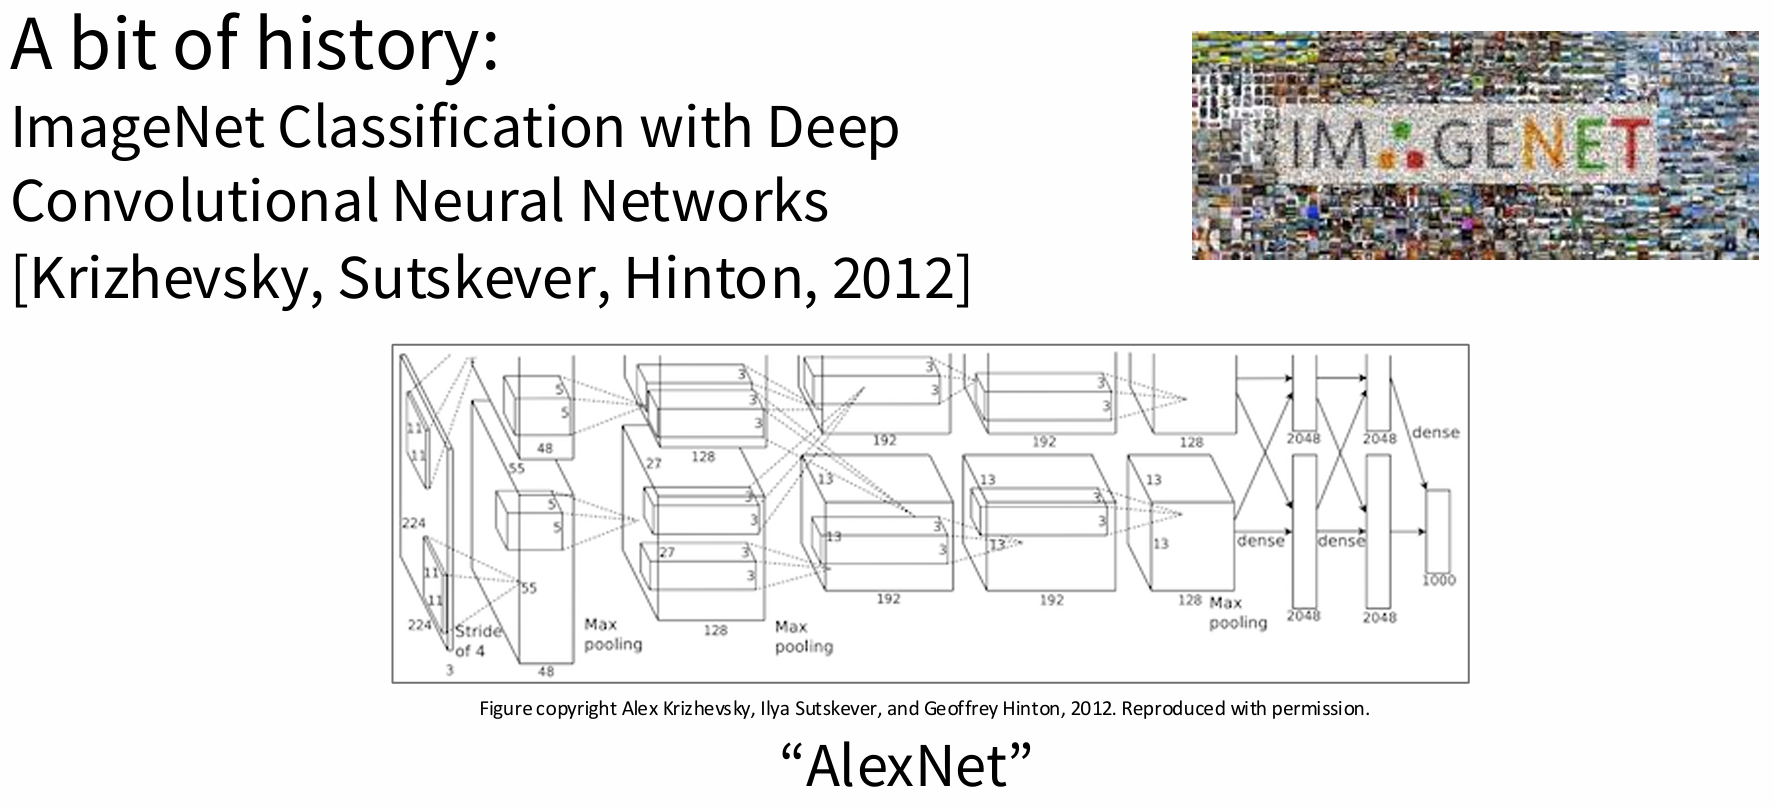
\includegraphics[width=1\textwidth]{images/intro_cnn.png}
	% Placeholder for: Basic CNN architecture showing Conv -> Pool -> FC
\end{frame}

\begin{frame}{CNN: History}


	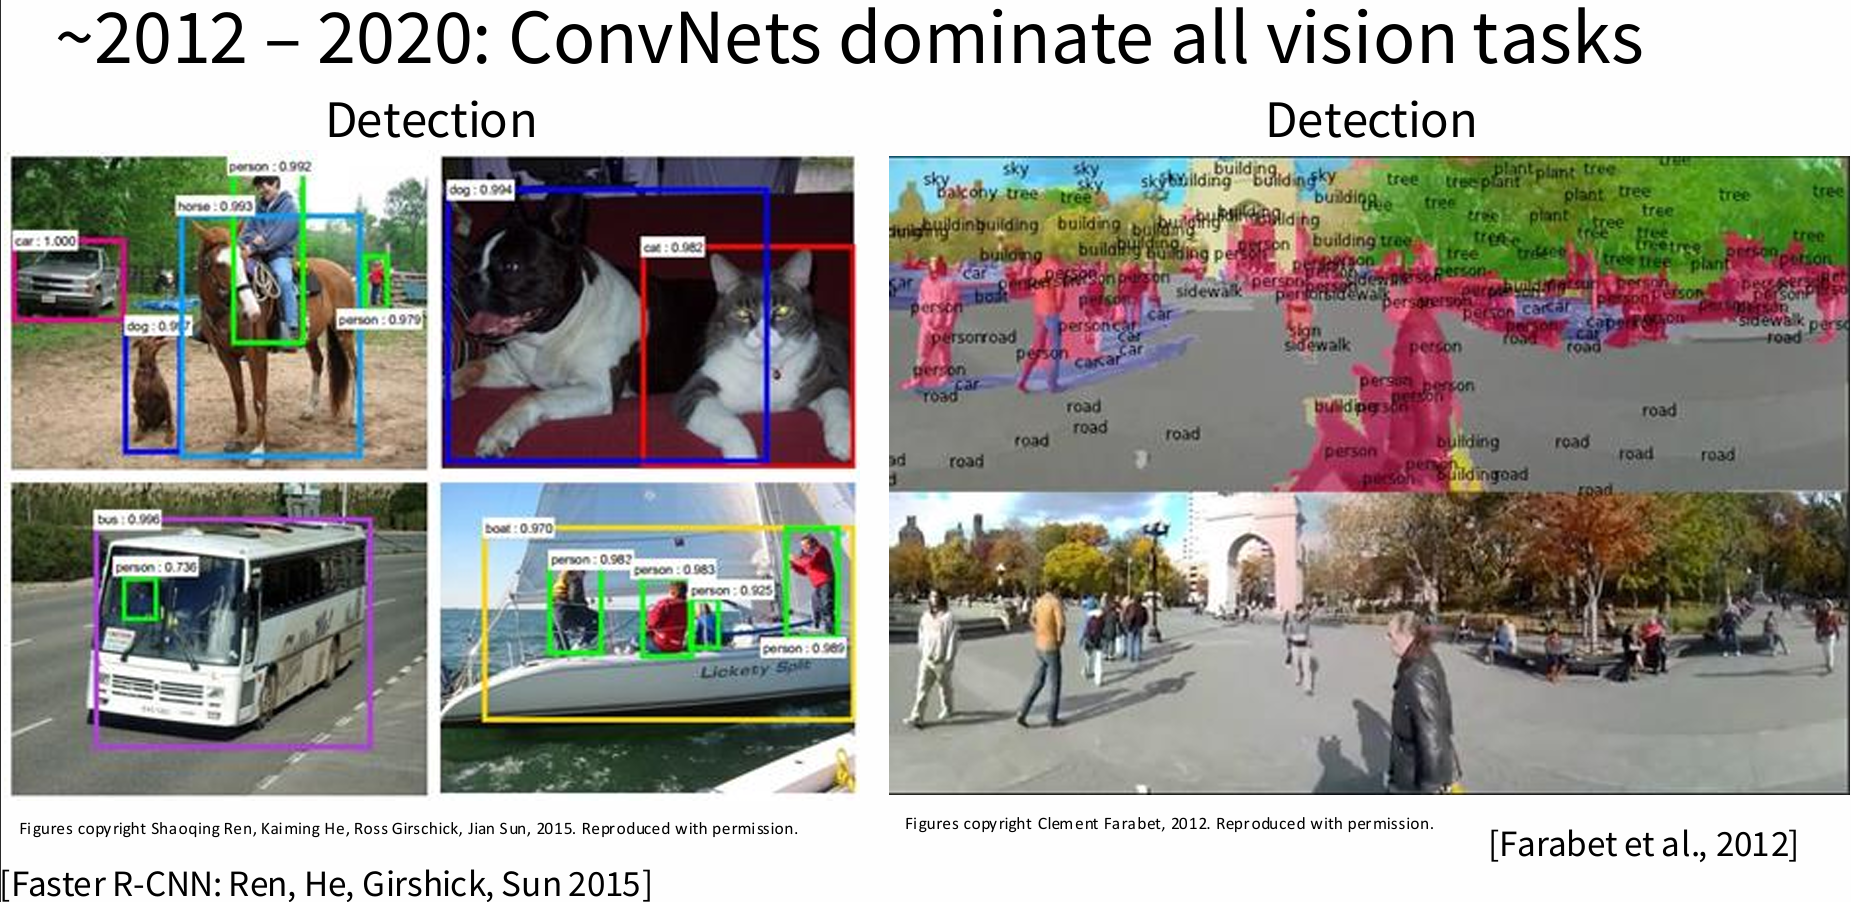
\includegraphics[width=1\textwidth]{images/intro_cnn2.png}
	% Placeholder for: Basic CNN architecture showing Conv -> Pool -> FC
\end{frame}

\begin{frame}{CNN: History}


	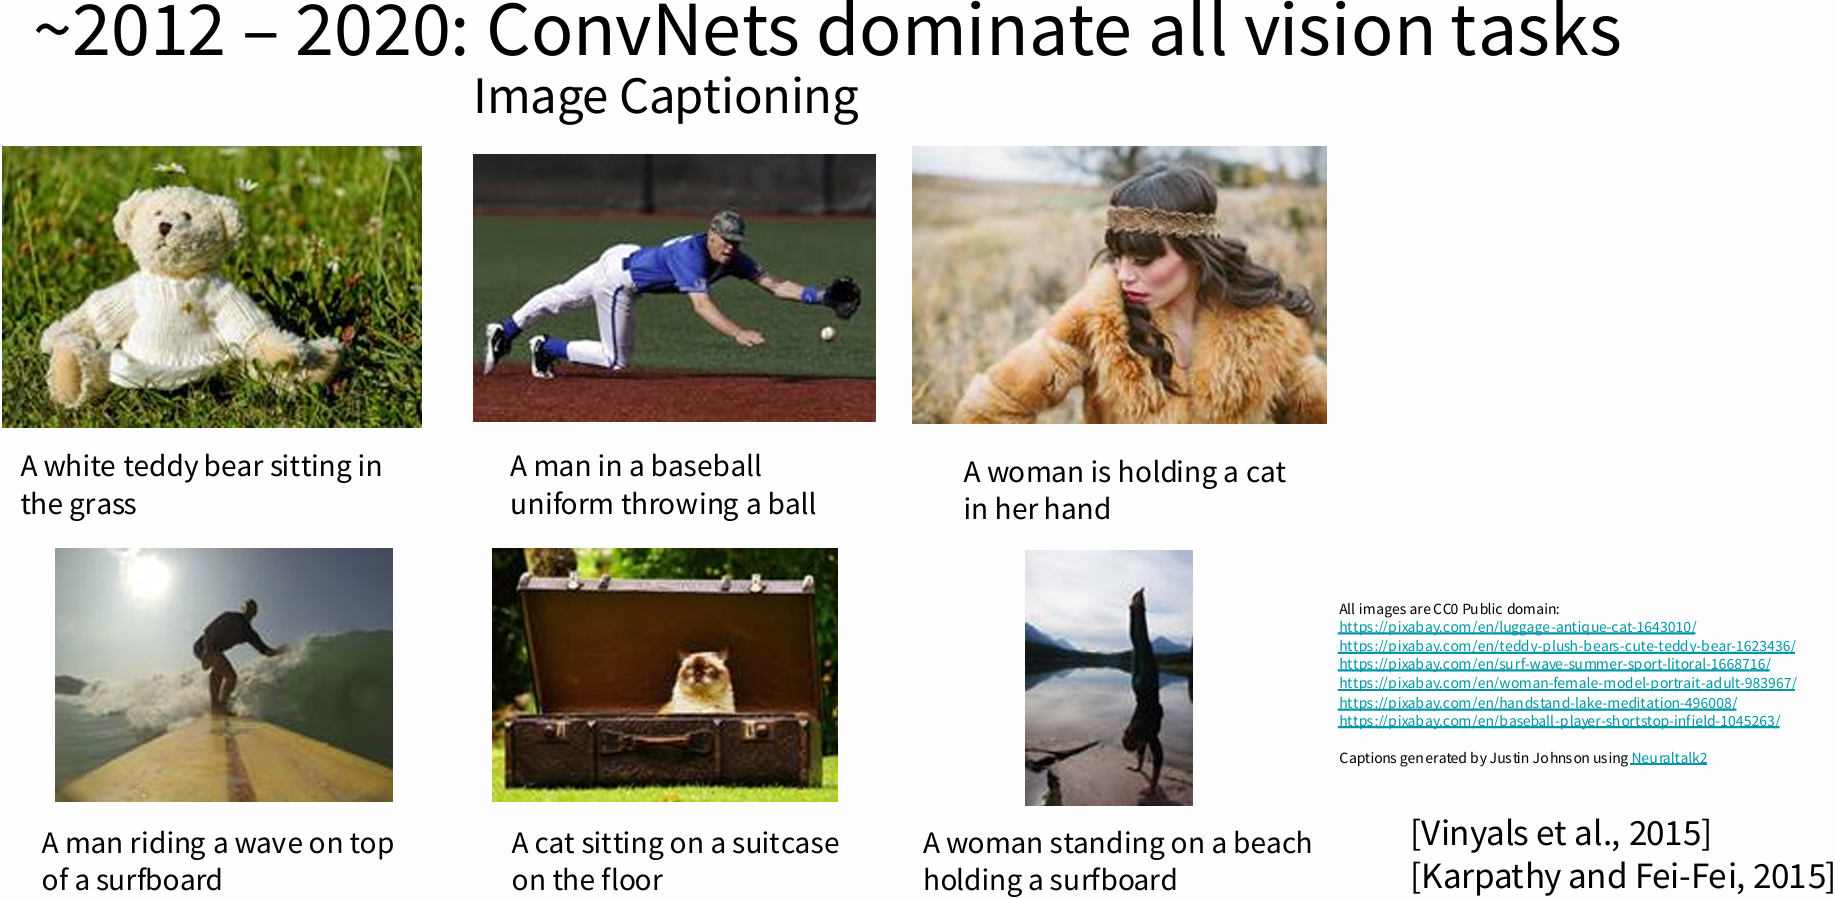
\includegraphics[width=1\textwidth]{images/intro_cnn3.png}
	% Placeholder for: Basic CNN architecture showing Conv -> Pool -> FC
\end{frame}

\begin{frame}{CNN: History}


	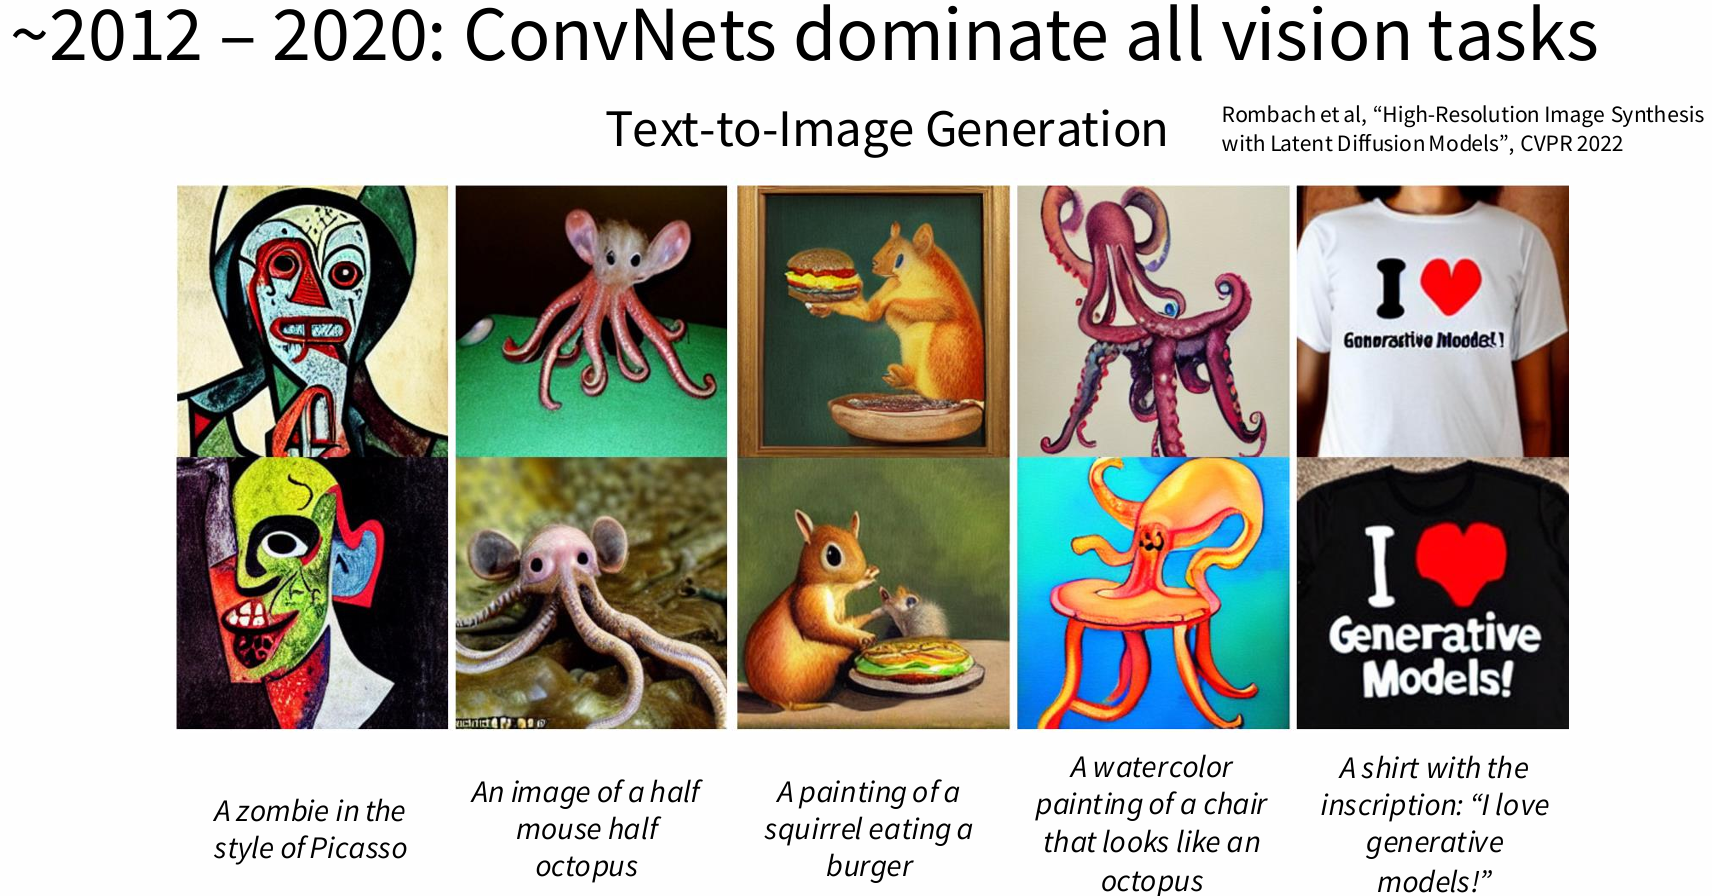
\includegraphics[width=1\textwidth]{images/intro_cnn4.png}
	% Placeholder for: Basic CNN architecture showing Conv -> Pool -> FC
\end{frame}

\begin{frame}{CNN: History}


	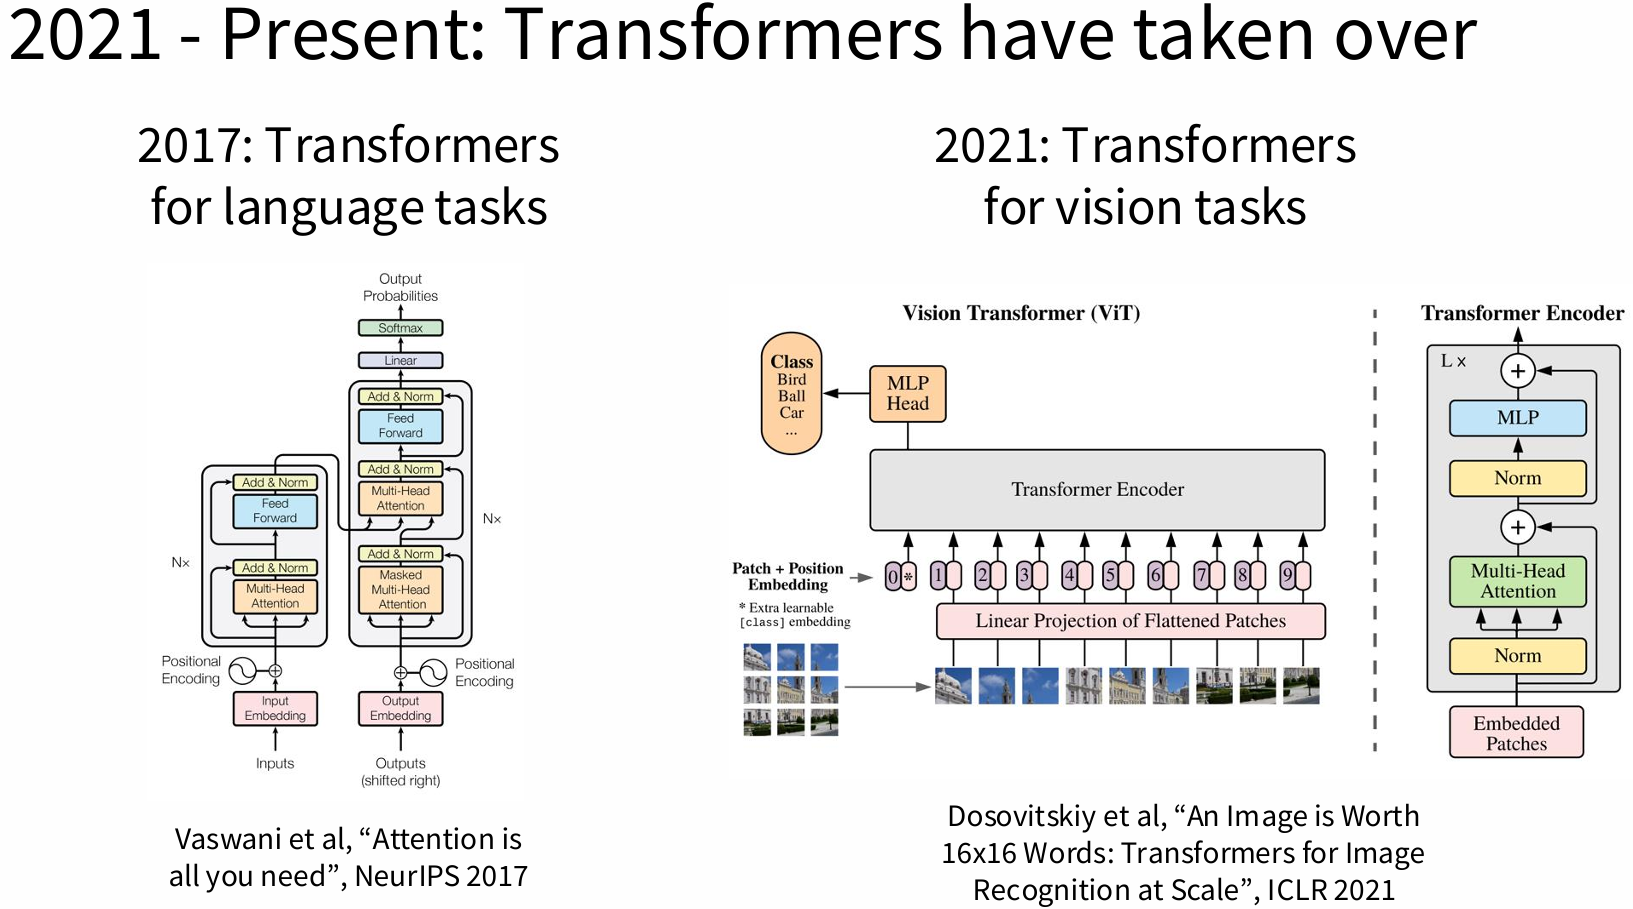
\includegraphics[width=1\textwidth]{images/intro_cnn5.png}
	% Placeholder for: Basic CNN architecture showing Conv -> Pool -> FC
\end{frame}


\begin{frame}{What is a Convolutional Neural Network (CNN)?}
	\begin{itemize}
		\item A type of Deep Learning model designed specifically for processing structured arrays of data, such as images.
		\item No need for features extraction.
	\end{itemize}
	\centering
	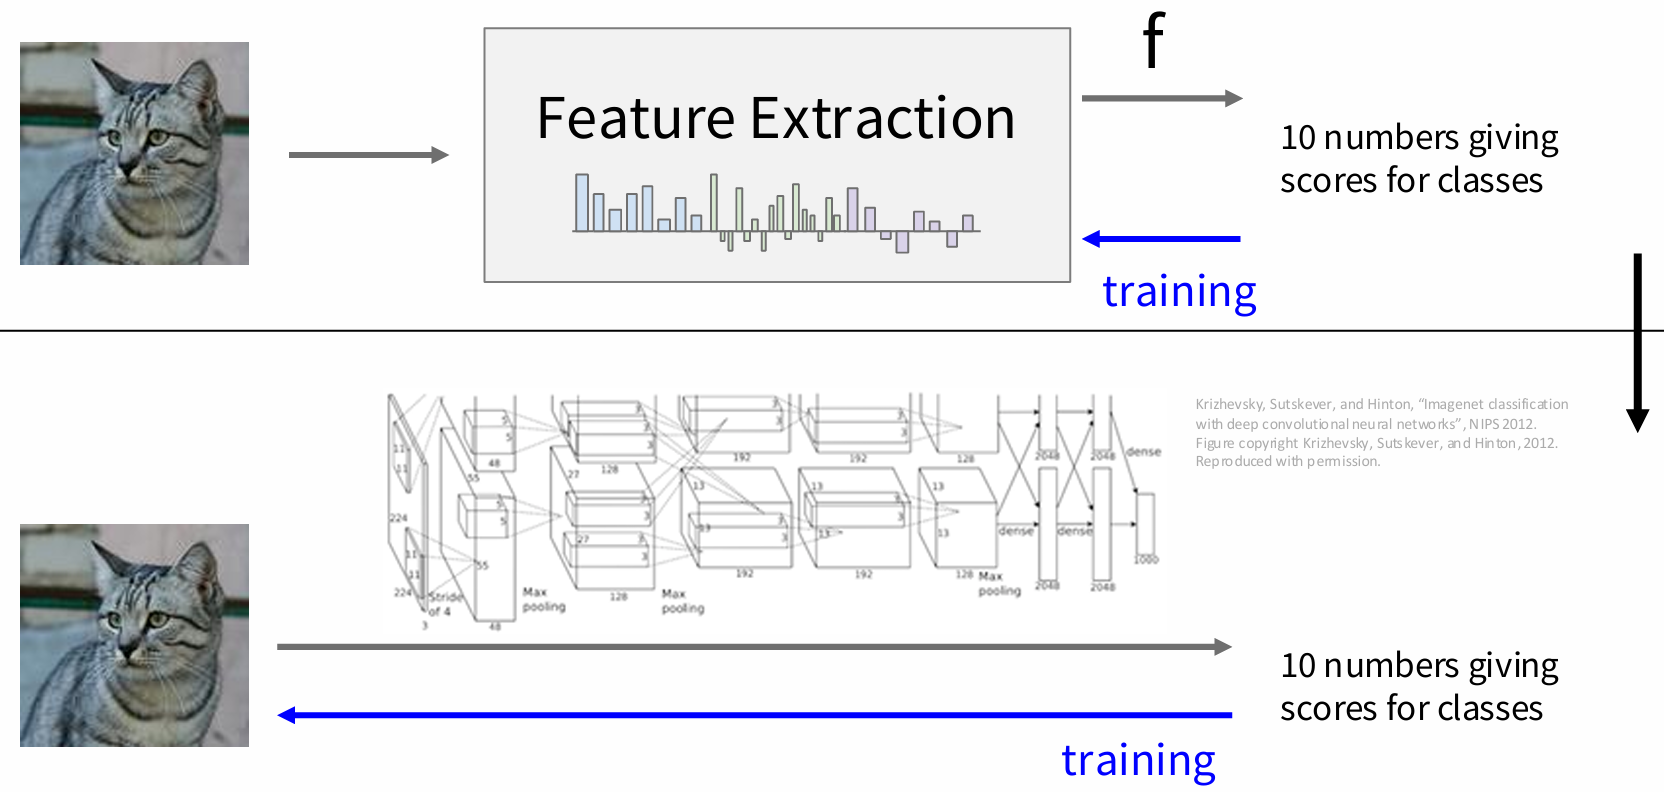
\includegraphics[width=0.8\textwidth]{images/cnn.png}
	% Placeholder for: Basic CNN architecture showing Conv -> Pool -> FC
\end{frame}

\begin{frame}{What is a Convolutional Neural Network (CNN)?}

	\centering
	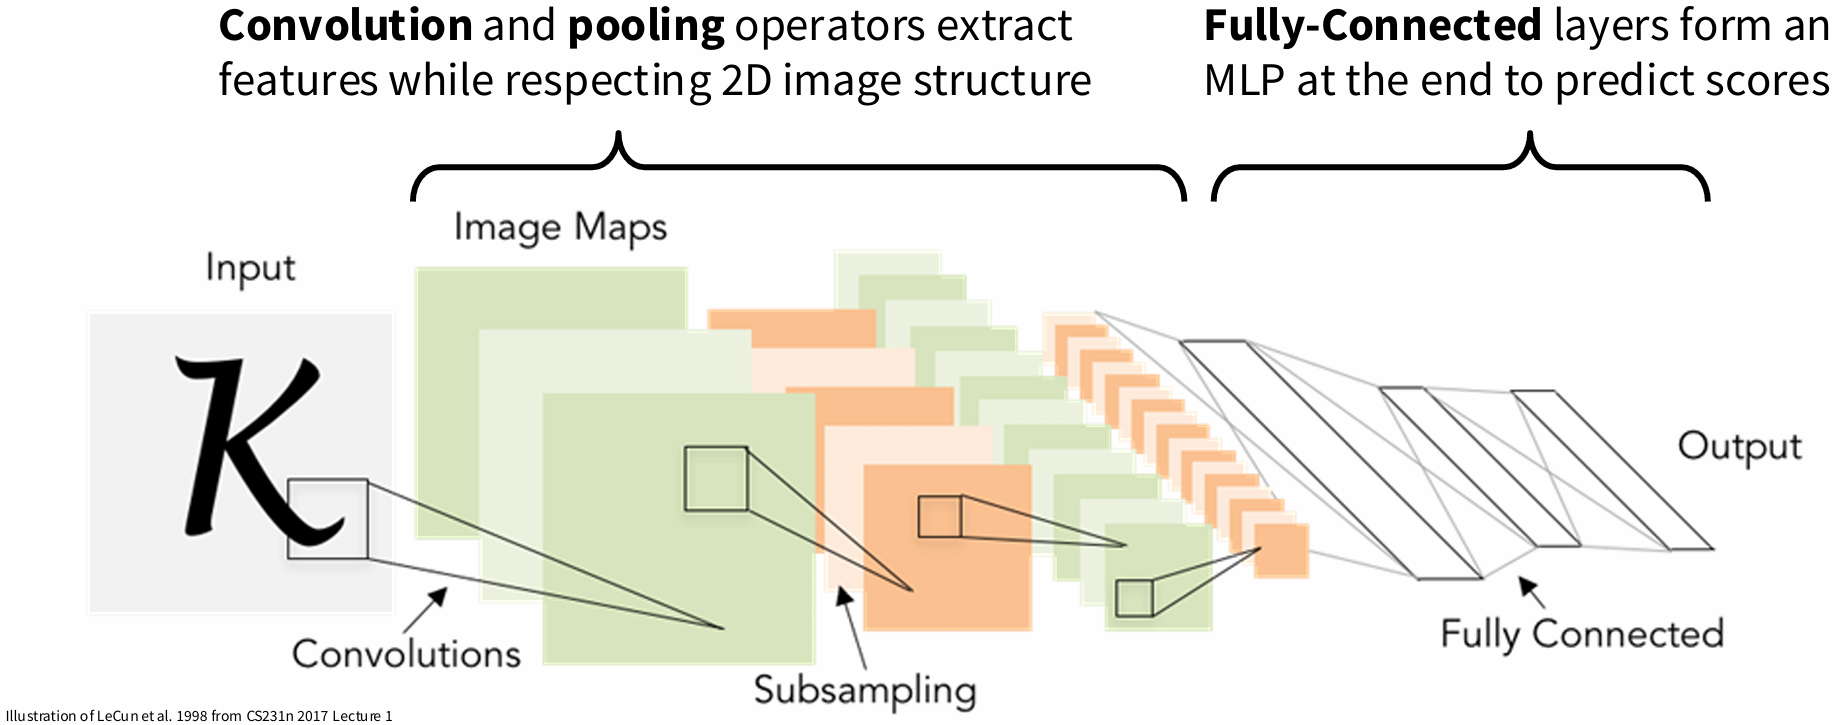
\includegraphics[width=1\textwidth]{images/cnn2.png}
	% Placeholder for: Basic CNN architecture showing Conv -> Pool -> FC
\end{frame}

\begin{frame}{The Convolution Operation}

	\begin{itemize}
			\item \textbf{Filters (Kernels):} Small matrices that slide across the image.
			\item \textbf{Feature Maps:} The result of the element-wise multiplication and summation.
		\end{itemize}
	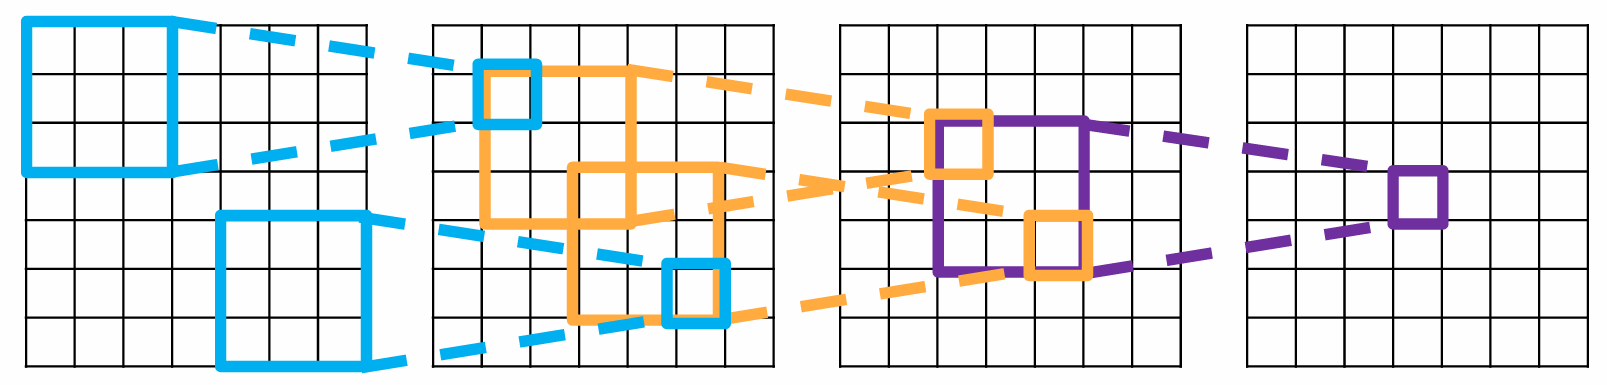
\includegraphics[width=1\textwidth]{images/cnn3.png}
	% Placeholder for: Basic CNN architecture showing Conv -> Pool -> FC
\end{frame}

\begin{frame}{The Convolution Operation}

	\begin{itemize}
			\item \textbf{Filters (Kernels):} Small matrices that slide across the image.
			\item \textbf{Feature Maps:} The result of the element-wise multiplication and summation.
		\end{itemize}
	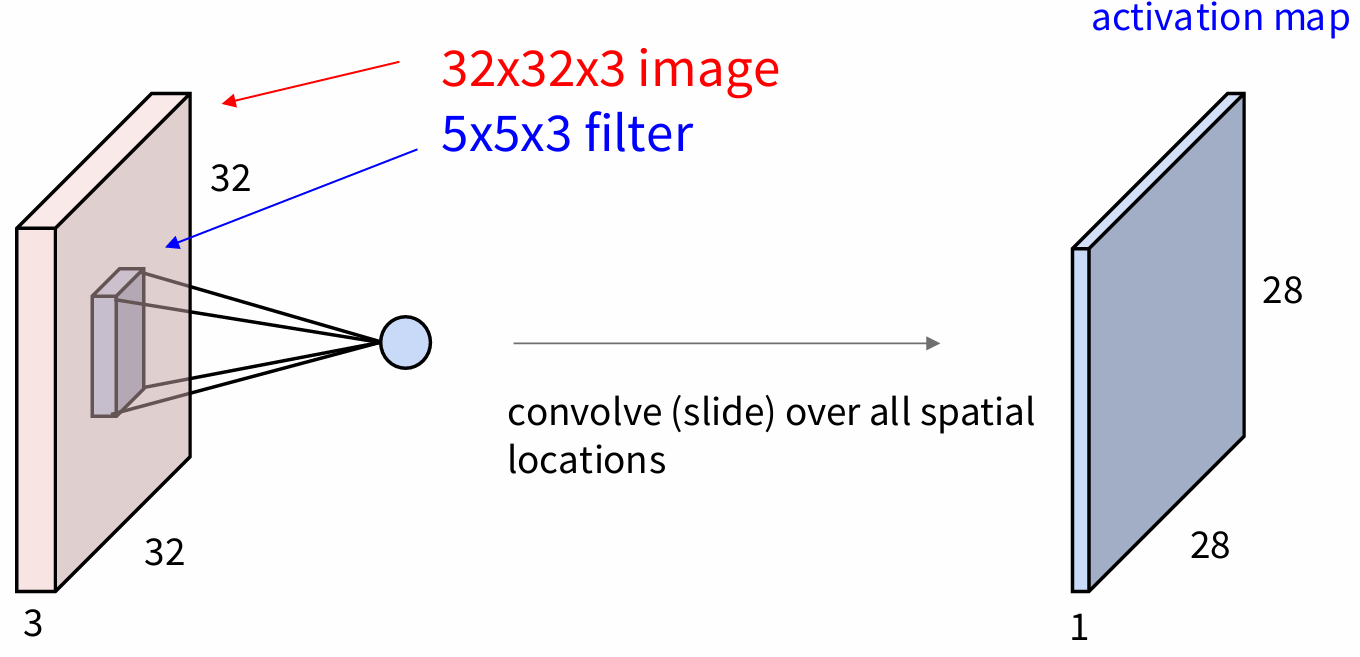
\includegraphics[width=0.9\textwidth]{images/cnn4.png}
	% Placeholder for: Basic CNN architecture showing Conv -> Pool -> FC
\end{frame}


\begin{frame}{The Convolution Operation}

	\begin{itemize}
			\item \textbf{Filters (Kernels):} Small matrices that slide across the image.
			\item \textbf{Feature Maps:} The result of the element-wise multiplication and summation.
		\end{itemize}
	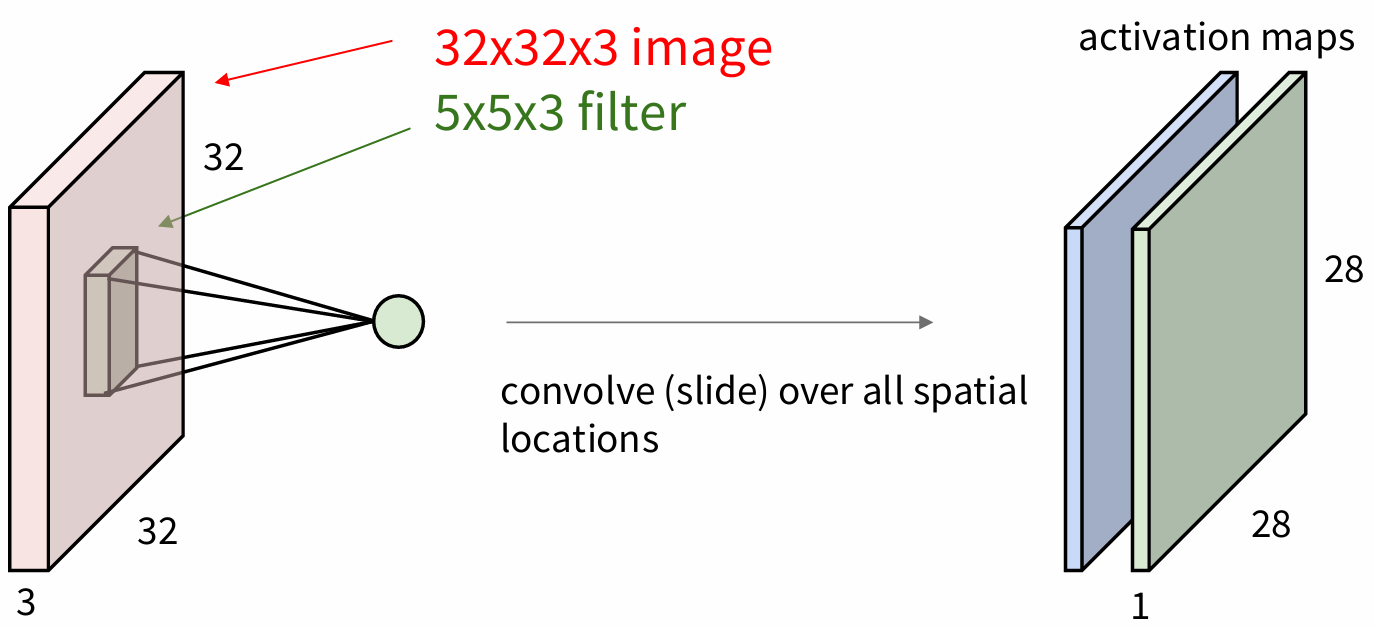
\includegraphics[width=0.9\textwidth]{images/cnn5.png}
	% Placeholder for: Basic CNN architecture showing Conv -> Pool -> FC
\end{frame}

\begin{frame}{From Features to Predictions}
	\begin{itemize}
		\item \textbf{Classifier:} Fully Connected (Dense) layers at the end.
		\item \textbf{Softmax:} Converts output scores into probabilities (for classification).
	\end{itemize}
	\centering
	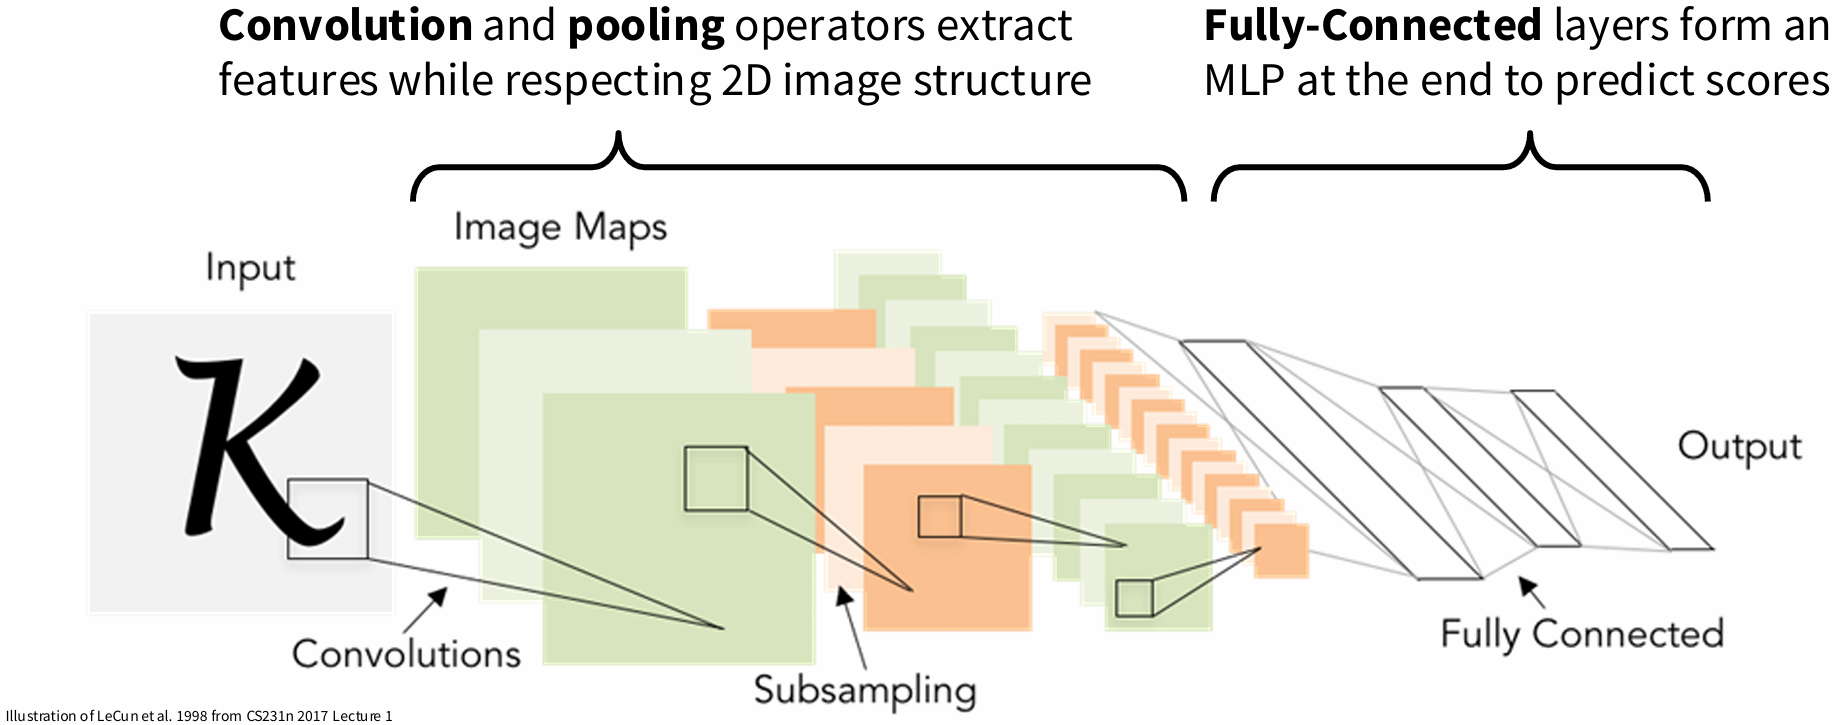
\includegraphics[width=0.8\textwidth]{images/cnn2.png}
	% Placeholder for: Basic CNN architecture showing Conv -> Pool -> FC
\end{frame}


\begin{frame}{Computer vision Tasks}
	\centering

	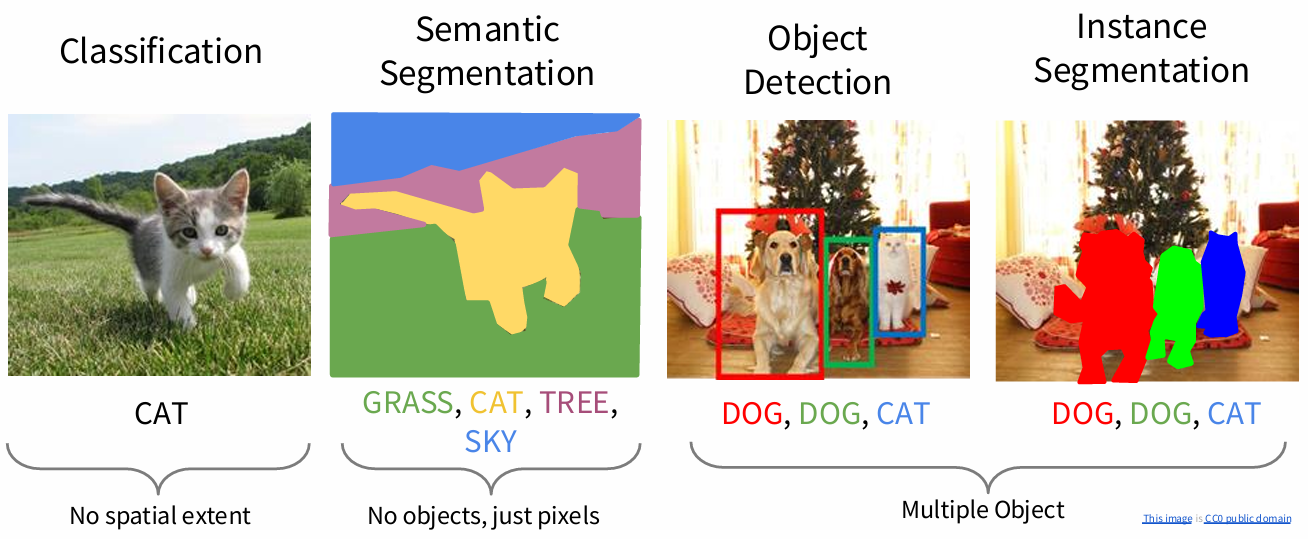
\includegraphics[width=1\textwidth]{images/cs_vision_tasks.png}
	% Placeholder for: A 3-panel image showing (L) Class, (M) Det, (R) Seg on the same anatomy
\end{frame}

\begin{frame}{Image classification}
	\centering

	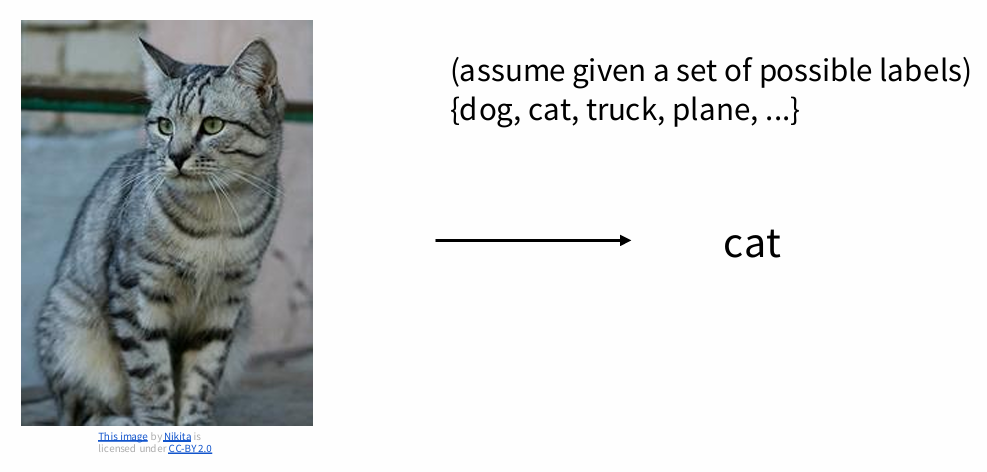
\includegraphics[width=1\textwidth]{images/intro_classification.png}
	% Placeholder for: A 3-panel image showing (L) Class, (M) Det, (R) Seg on the same anatomy
\end{frame}

% ============================================================
\section{Semantic Segmentation}
% ============================================================


\begin{frame}{Semantic Segmentation}
	\centering

	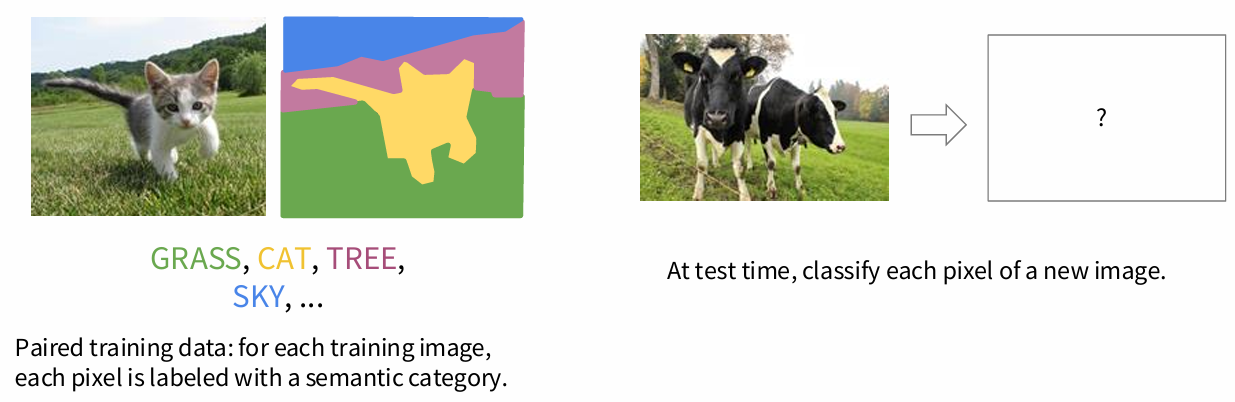
\includegraphics[width=1\textwidth]{images/intro_semantic.png}
	% Placeholder for: A 3-panel image showing (L) Class, (M) Det, (R) Seg on the same anatomy
\end{frame}

\begin{frame}{Semantic Segmentation}
	\begin{columns}
		\column{0.4\textwidth}
		\begin{itemize}
			\item \textbf{Pixel-level Detail:} Assigns a class to every pixel.
			\item It don't understand about instance.
		\end{itemize}
		\column{0.6\textwidth}
		\centering
		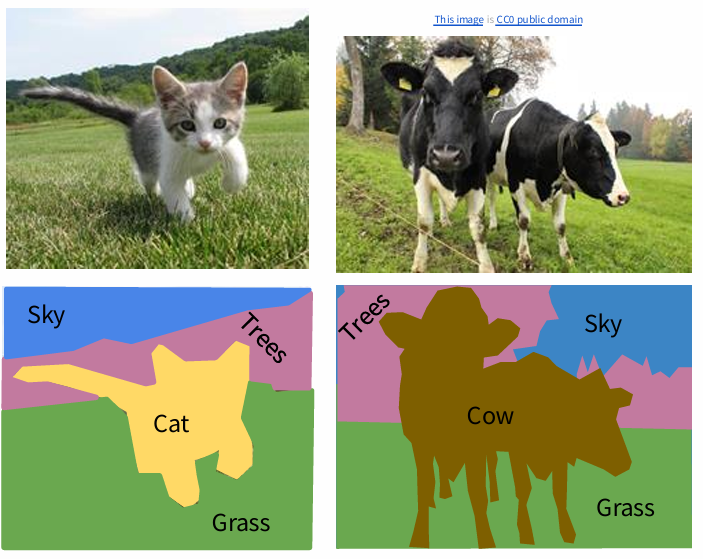
\includegraphics[width=\textwidth]{images/intro_semantic2.png}
	\end{columns}
\end{frame}

\begin{frame}{Semantic Segmentation: Fully Convolutional Networks}
	\centering
	\begin{itemize}
		\item Use convolutions
		\item Use upsampling
	\end{itemize}
	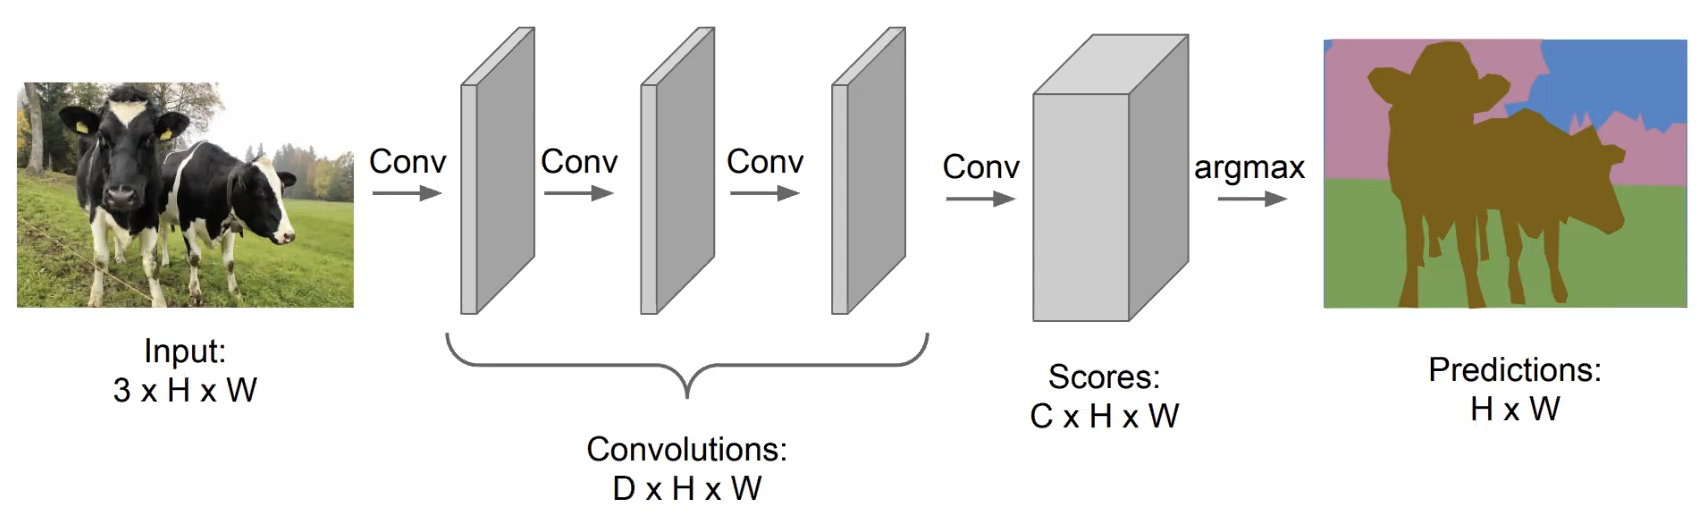
\includegraphics[width=1\textwidth]{images/semantic.png}
	% Placeholder for: A 3-panel image showing (L) Class, (M) Det, (R) Seg on the same anatomy
\end{frame}

\begin{frame}{Semantic Segmentation: Learning Deconvolution Network}
	\centering
	\begin{itemize}
		\item Instead of abruptly upsampling, we gradually upsample.
		\item Learn upsampling filters.
	\end{itemize}
	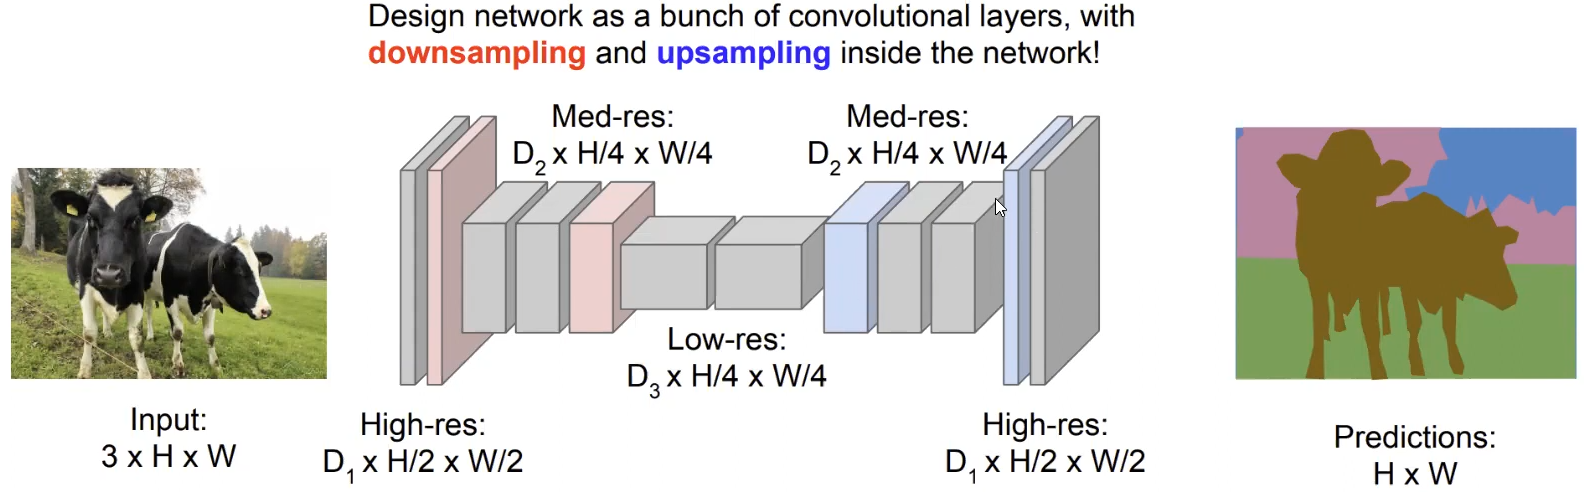
\includegraphics[width=1\textwidth]{images/semantic2.png}
	% Placeholder for: A 3-panel image showing (L) Class, (M) Det, (R) Seg on the same anatomy
\end{frame}

\begin{frame}{Semantic Segmentation: UNet}
	\begin{columns}
		\column{0.4\textwidth}
		\begin{itemize}
			\item Use multi-scale features
			\item Skip connections
		\end{itemize}
		\column{0.6\textwidth}
		\centering
		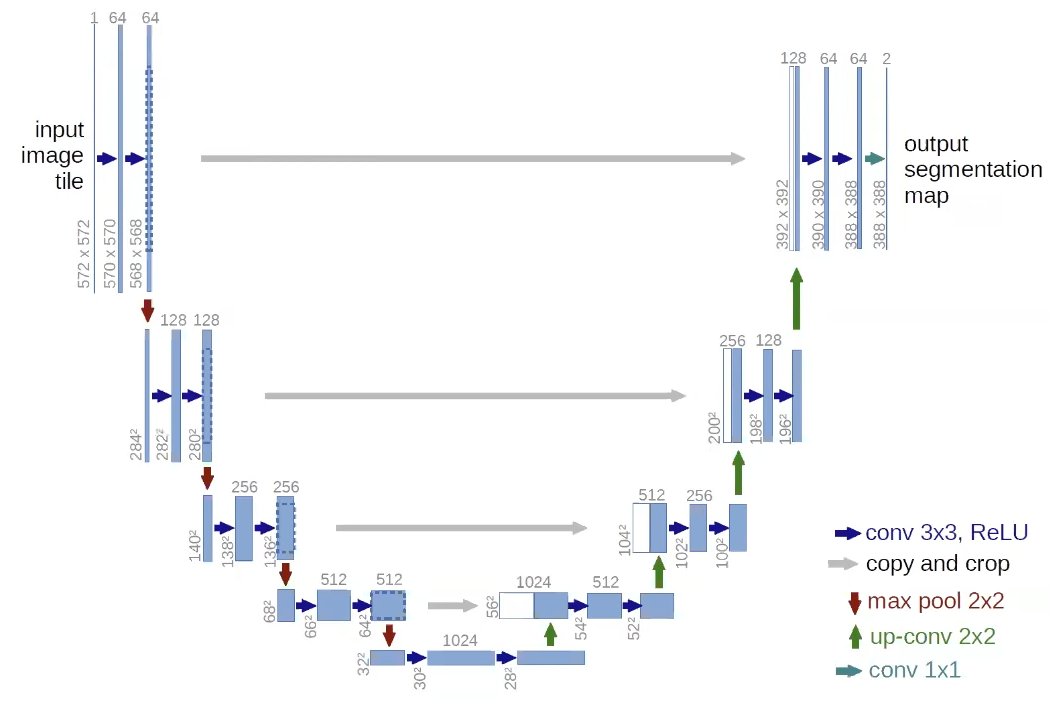
\includegraphics[width=\textwidth]{images/semantic_unet.png}
	\end{columns}
\end{frame}



% ============================================================
\section{Image Detection}
% ============================================================
\begin{frame}{Introduction to Object Detection}
	\begin{columns}
		\column{0.5\textwidth}
		\begin{itemize}
			\item \textbf{Task:} Identify and locate objects of interest.
			\item \textbf{Output:} Class + Bounding Box $(x, y, w, h)$.
			\item \textbf{Medical Examples:}
			      \begin{itemize}
				      \item Lung nodules in CT.
				      \item Landmarks for radiotherapy.
			      \end{itemize}
		\end{itemize}
		\column{0.5\textwidth}
		\centering
		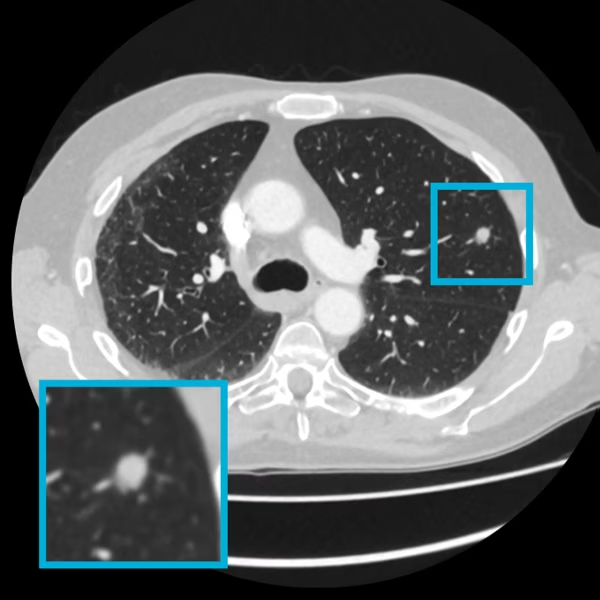
\includegraphics[width=\textwidth]{images/detection.png}
		% Placeholder for: CT image with bounding boxes around nodules
	\end{columns}
\end{frame}


\begin{frame}{Object Detection: Single Object}
	\centering

	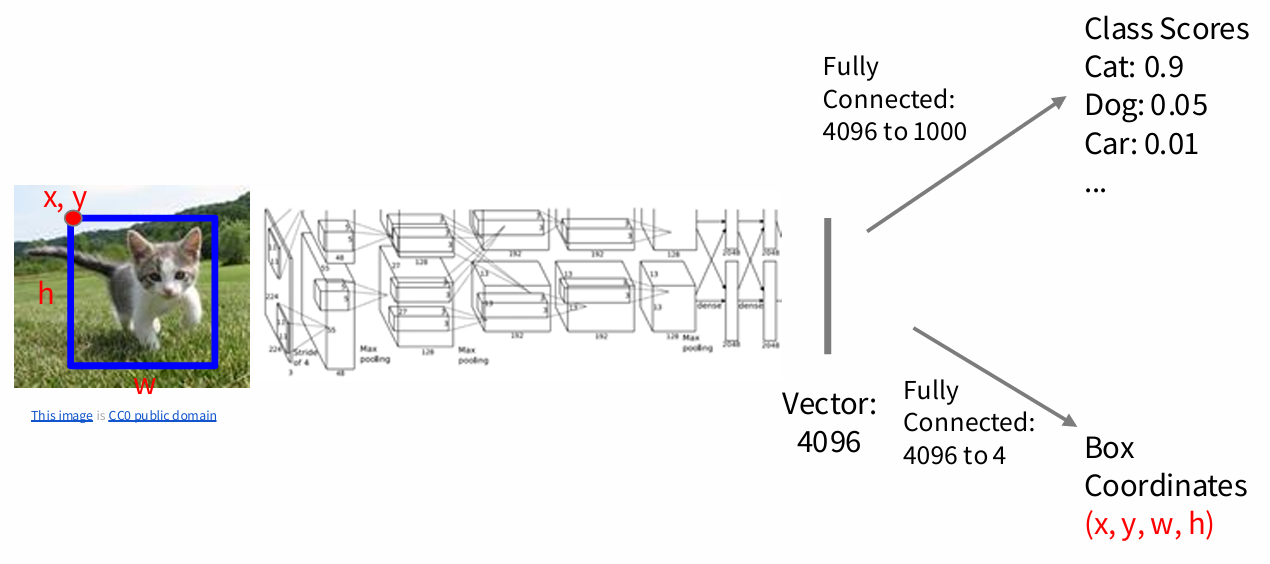
\includegraphics[width=1\textwidth]{images/intro_detection.png}
	% Placeholder for: A 3-panel image showing (L) Class, (M) Det, (R) Seg on the same anatomy
\end{frame}


\begin{frame}{Object Detection: Multiple Objects}
	\centering

	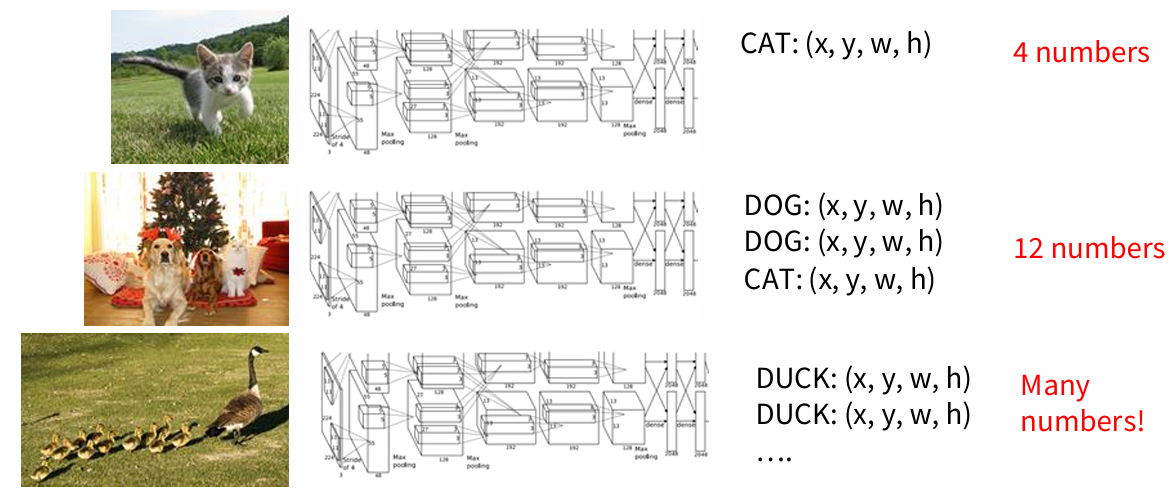
\includegraphics[width=1\textwidth]{images/intro_detection2.png}
	% Placeholder for: A 3-panel image showing (L) Class, (M) Det, (R) Seg on the same anatomy
\end{frame}


\begin{frame}{Object Detection: Multiple Objects}
	\centering

	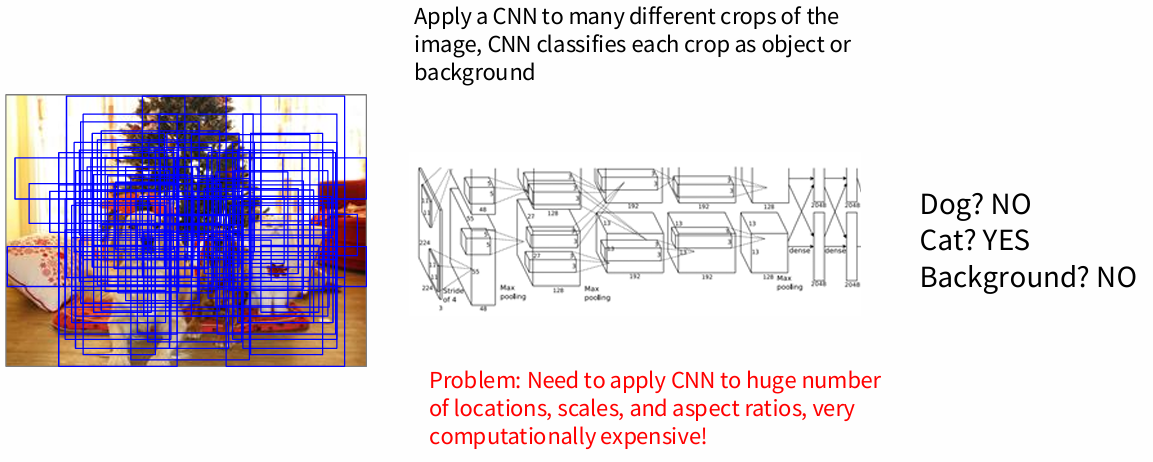
\includegraphics[width=1\textwidth]{images/intro_detection3.png}
	% Placeholder for: A 3-panel image showing (L) Class, (M) Det, (R) Seg on the same anatomy
\end{frame}


\begin{frame}{Two Main Paradigms in Detection}
	\begin{columns}
		\column{0.5\textwidth}
		\textbf{Two-Stage Detectors}
		\begin{itemize}
			\item Step 1: Propose regions.
			\item Step 2: Classify and refine.
			\item \textit{Example:} \textbf{R-CNN}.
			\item Accuracy is high, but slower.
		\end{itemize}

		\column{0.5\textwidth}
		\textbf{One-Stage Detectors}
		\begin{itemize}
			\item Direct prediction in one go.
			\item \textit{Example:} \textbf{YOLO (You Only Look Once)}.
			\item Extremely fast, suitable for real-time applications (e.g., ultrasound).
		\end{itemize}
	\end{columns}
\end{frame}

\begin{frame}{Two-Stage Detectors: R-CNN, Region Proposals}
	\centering
	\begin{itemize}
		\item Use traditional method to propose regions: Selective Search.
		\item Selective Search gives 2000 region proposals in a few seconds on CPU.
		\item This algorithm use in both \textbf{R-CNN and Fast R-CNN}.
	\end{itemize}
	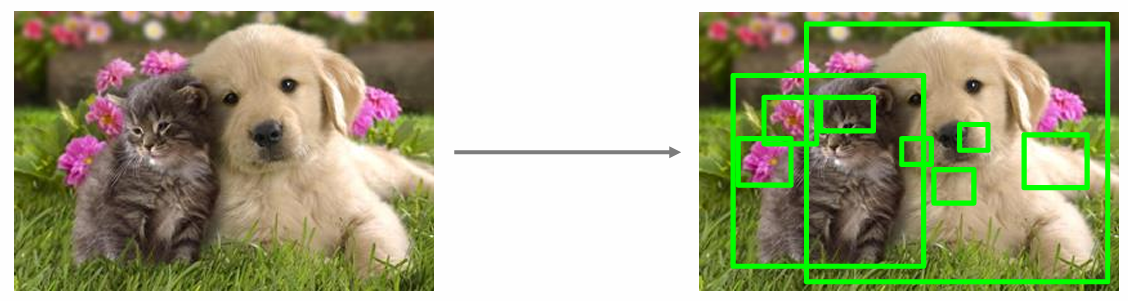
\includegraphics[width=1\textwidth]{images/rcnn.png}
	% Placeholder for: A 3-panel image showing (L) Class, (M) Det, (R) Seg on the same anatomy
\end{frame}

\begin{frame}{Two-Stage Detectors: R-CNN}
	\centering

	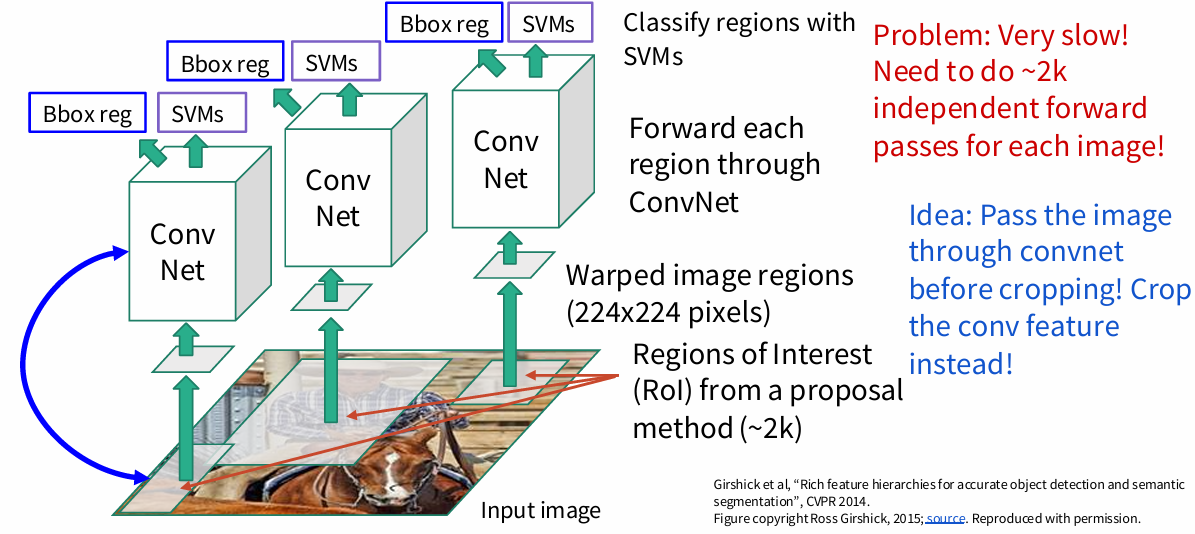
\includegraphics[width=1\textwidth]{images/rcnn2.png}
	% Placeholder for: A 3-panel image showing (L) Class, (M) Det, (R) Seg on the same anatomy
\end{frame}

\begin{frame}{Two-Stage Detectors: Fast R-CNN}
	\centering

	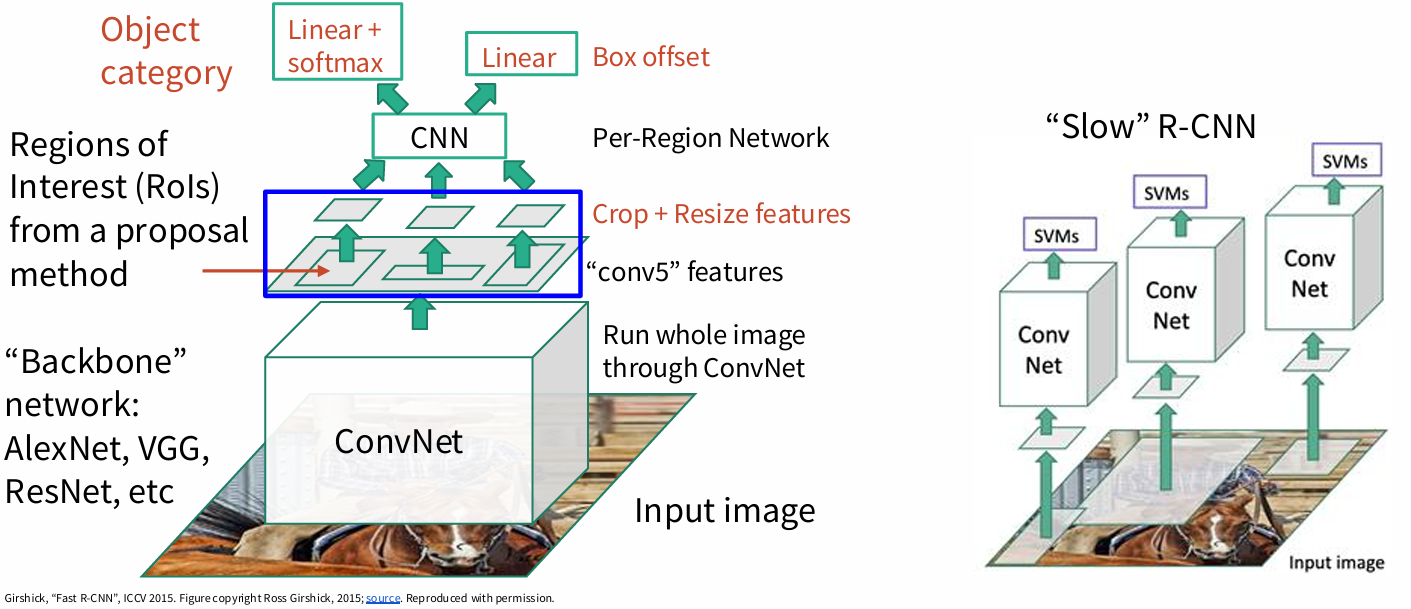
\includegraphics[width=1\textwidth]{images/fast_rcnn.png}
	% Placeholder for: A 3-panel image showing (L) Class, (M) Det, (R) Seg on the same anatomy
\end{frame}

\begin{frame}{Two-Stage Detectors: Fast R-CNN}
	\centering

	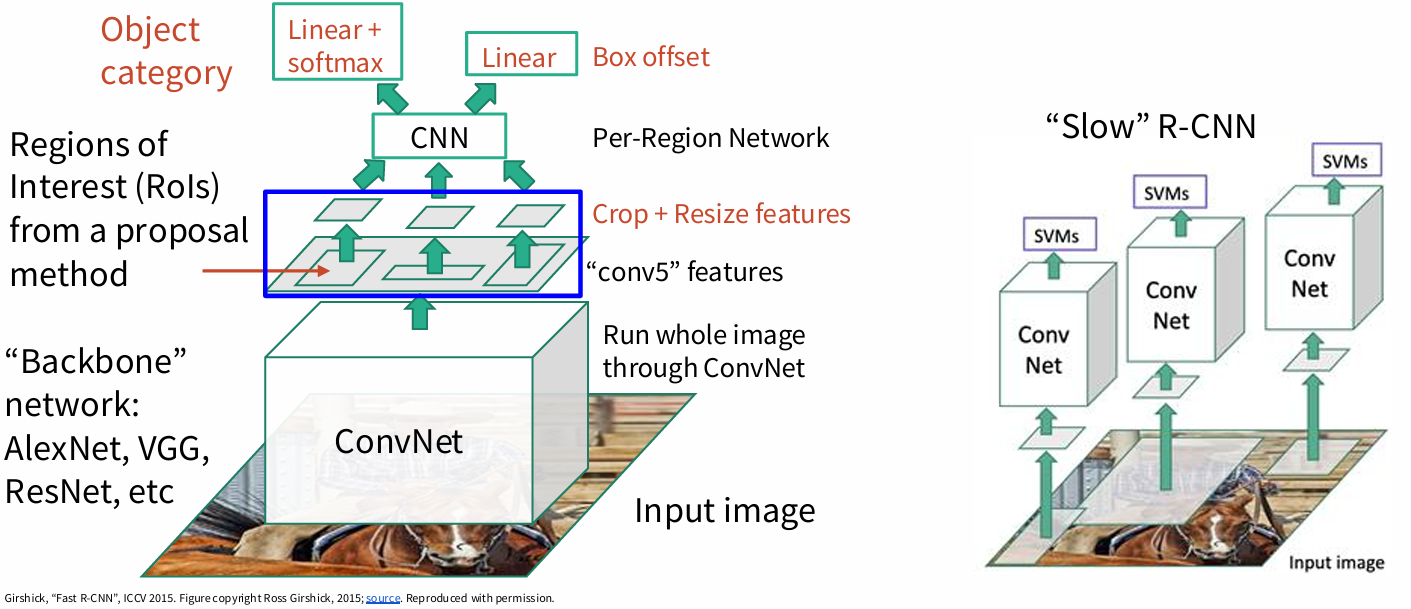
\includegraphics[width=1\textwidth]{images/fast_rcnn.png}
	% Placeholder for: A 3-panel image showing (L) Class, (M) Det, (R) Seg on the same anatomy
\end{frame}



\begin{frame}{Two-Stage Detectors}
	\centering

	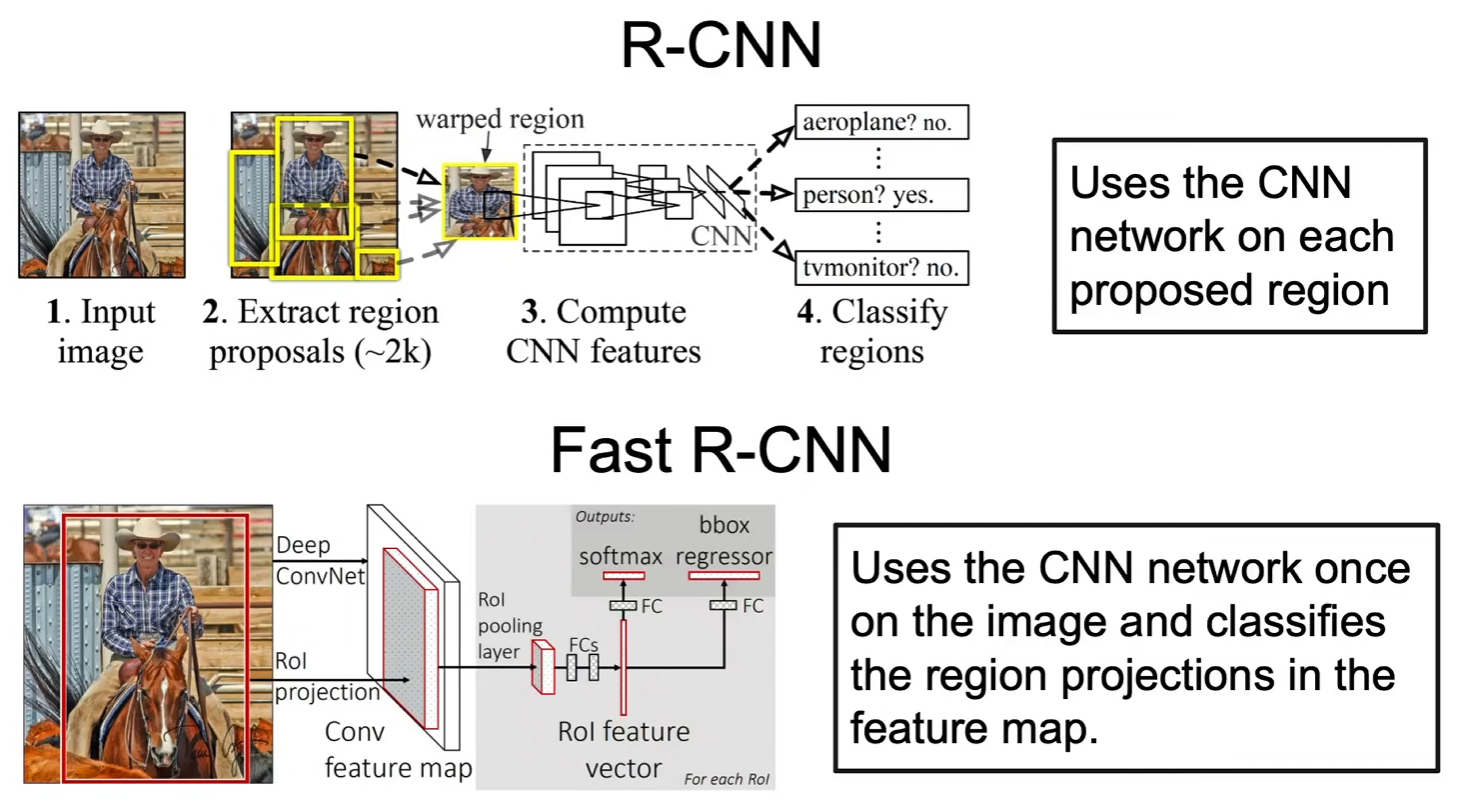
\includegraphics[width=1\textwidth]{images/rcnn_summary.png}
	% Placeholder for: A 3-panel image showing (L) Class, (M) Det, (R) Seg on the same anatomy
\end{frame}

\begin{frame}{Two-Stage Detectors: Fast R-CNN issue}

	\centering

	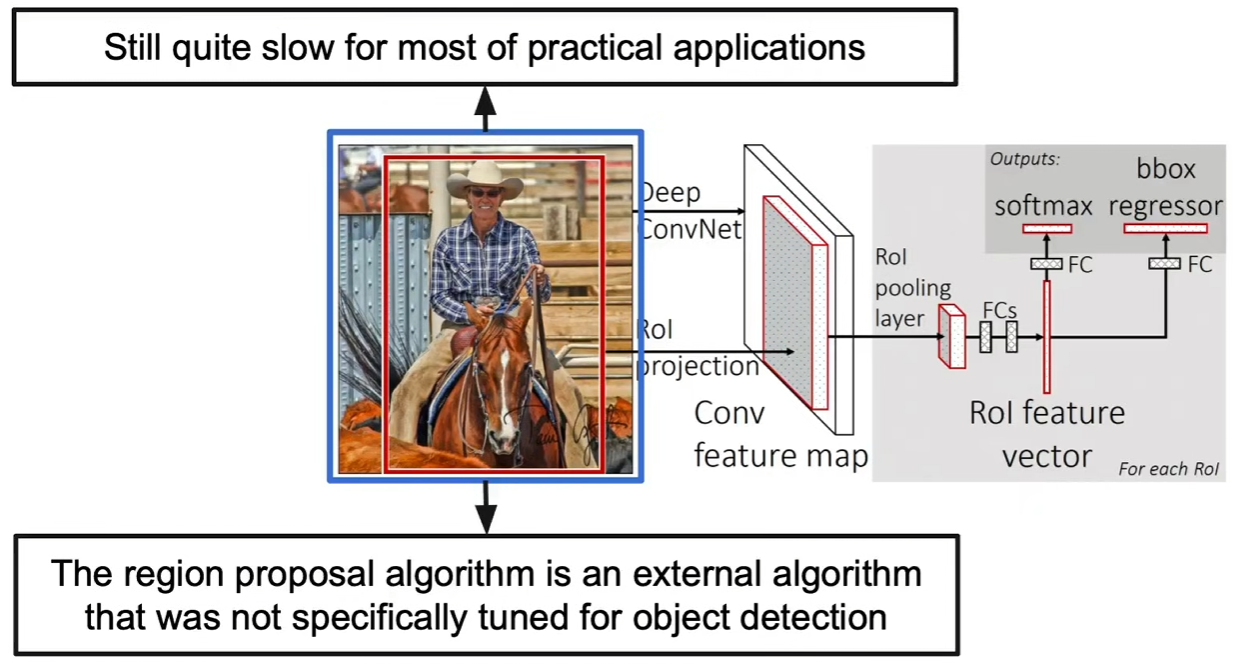
\includegraphics[width=1\textwidth]{images/faster_rcnn.png}
	% Placeholder for: A 3-panel image showing (L) Class, (M) Det, (R) Seg on the same anatomy
\end{frame}

\begin{frame}{Two-Stage Detectors: Faster R-CNN}

	\begin{columns}
		\column{0.5\textwidth}
		\begin{itemize}
			\item Region Proposal Network (RPN) trained to produce region proposals directly.
			\item After RPN, everything is the same as Fast R-CNN
		\end{itemize}
		\column{0.5\textwidth}

		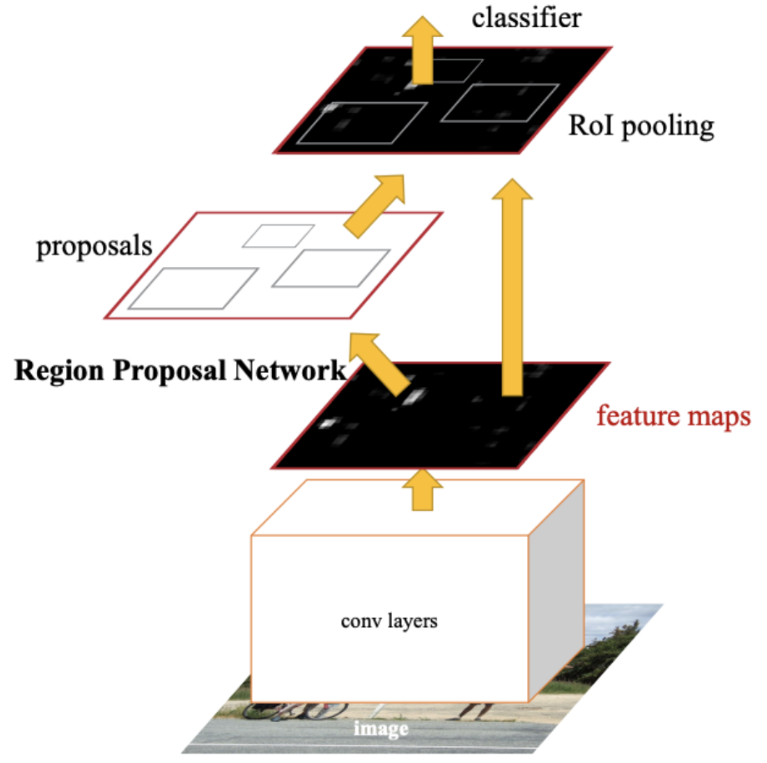
\includegraphics[width=\textwidth]{images/faster_rcnn2.png}
		% Placeholder for: CT image with bounding boxes around nodules
	\end{columns}

	% Placeholder for: A 3-panel image showing (L) Class, (M) Det, (R) Seg on the same anatomy
\end{frame}

\begin{frame}{Two-Stage Detectors: Faster R-CNN}

	\centering

	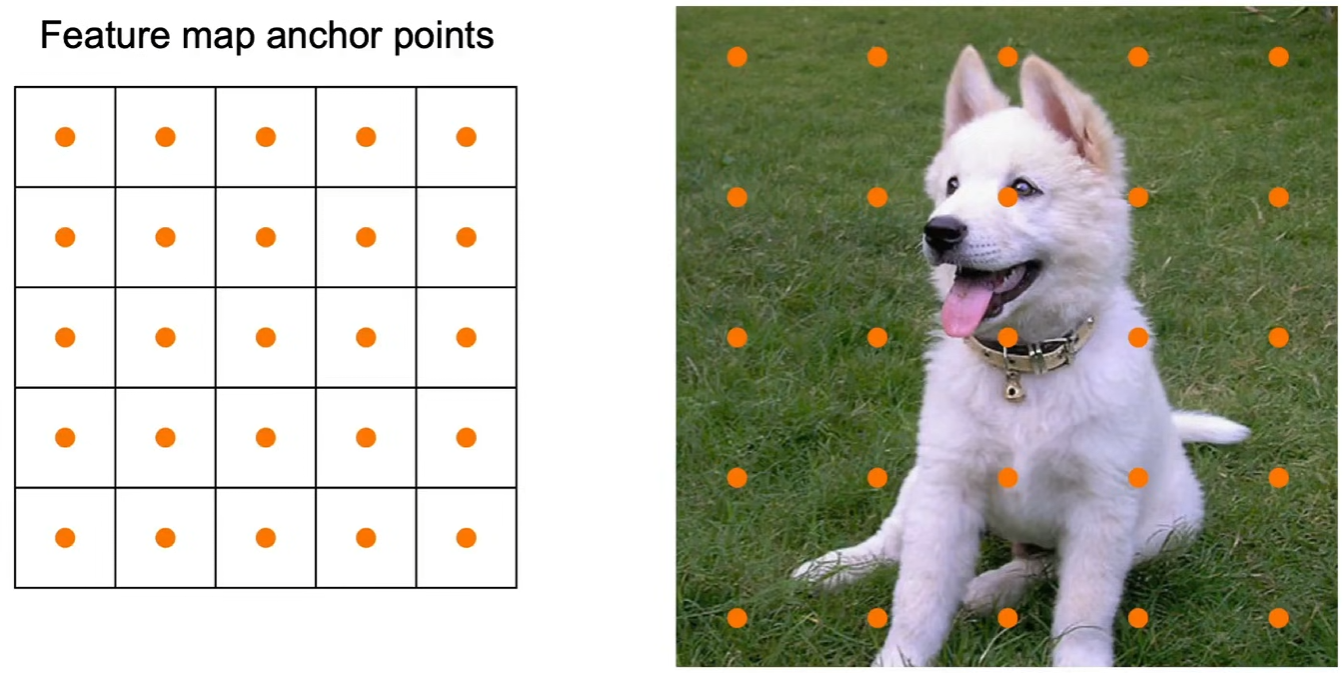
\includegraphics[width=1\textwidth]{images/faster_rcnn_anchor.png}
	% Placeholder for: A 3-panel image showing (L) Class, (M) Det, (R) Seg on the same anatomy
\end{frame}

\begin{frame}{Two-Stage Detectors: Faster R-CNN RPN}

	\begin{columns}
		\column{0.35\textwidth}
		\begin{itemize}
			\item Fix the number of proposals by using a set of k = 9 anchors per location.
			\item After RPN, everything is the same as Fast R-CNN
		\end{itemize}
		\column{0.65\textwidth}
		\centering
		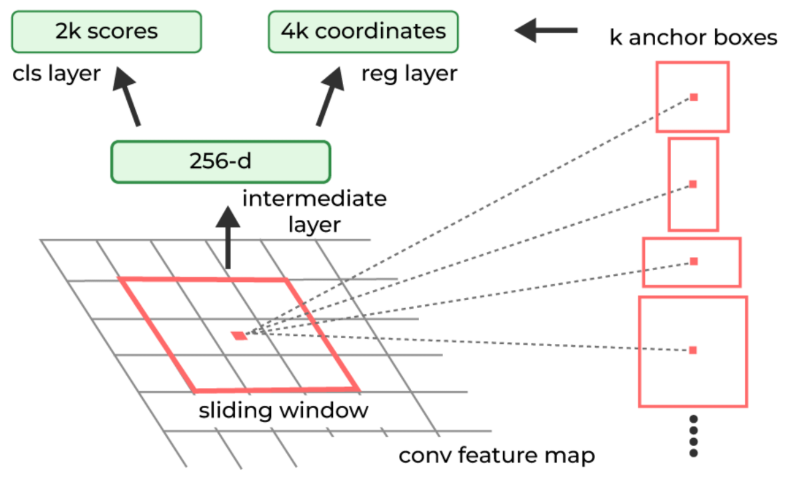
\includegraphics[width=\textwidth]{images/faster_rcnn_rpn.png}
		% Placeholder for: CT image with bounding boxes around nodules
	\end{columns}
	% Placeholder for: A 3-panel image showing (L) Class, (M) Det, (R) Seg on the same anatomy
\end{frame}

\begin{frame}{Two-Stage Detectors: Faster R-CNN RPN}

	\centering

	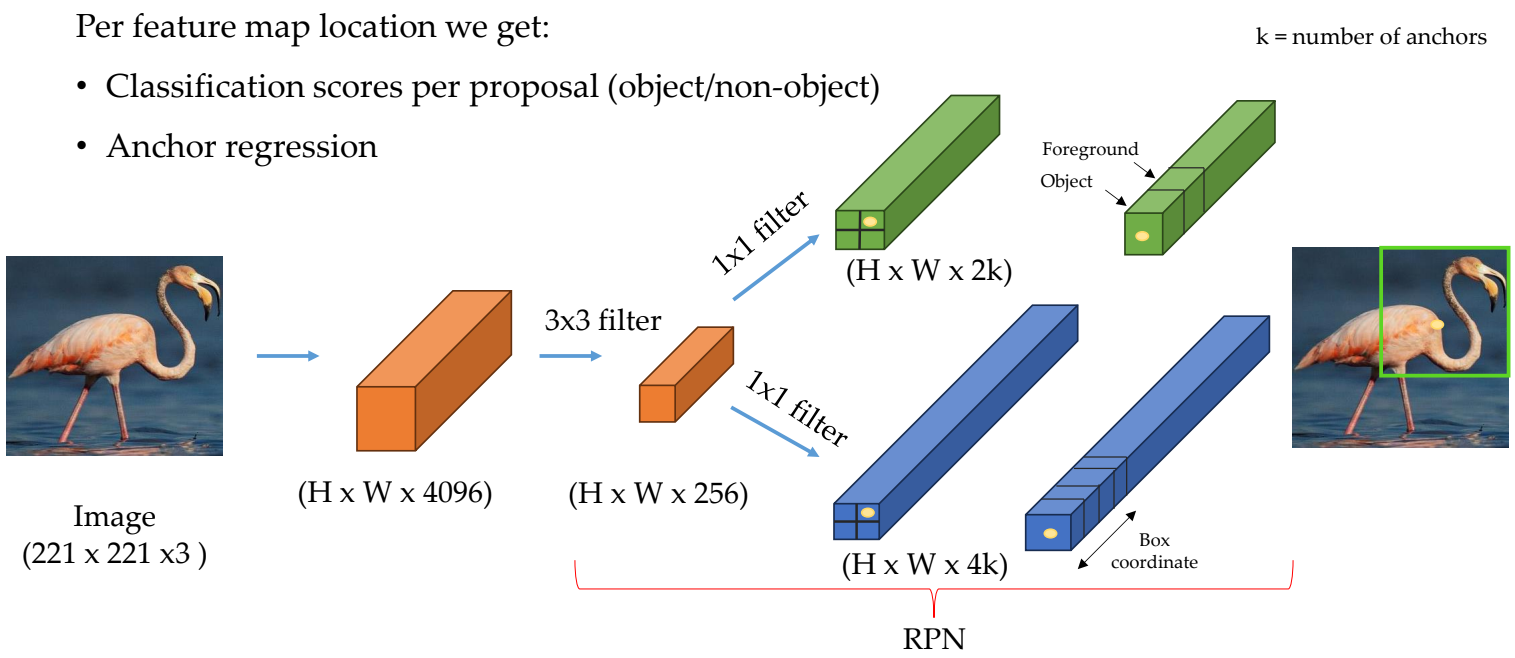
\includegraphics[width=1\textwidth]{images/faster_rcnn_rpn2.png}
	% Placeholder for: A 3-panel image showing (L) Class, (M) Det, (R) Seg on the same anatomy
\end{frame}

\begin{frame}{Two-Stage Detectors: Faster R-CNN}

	\centering

	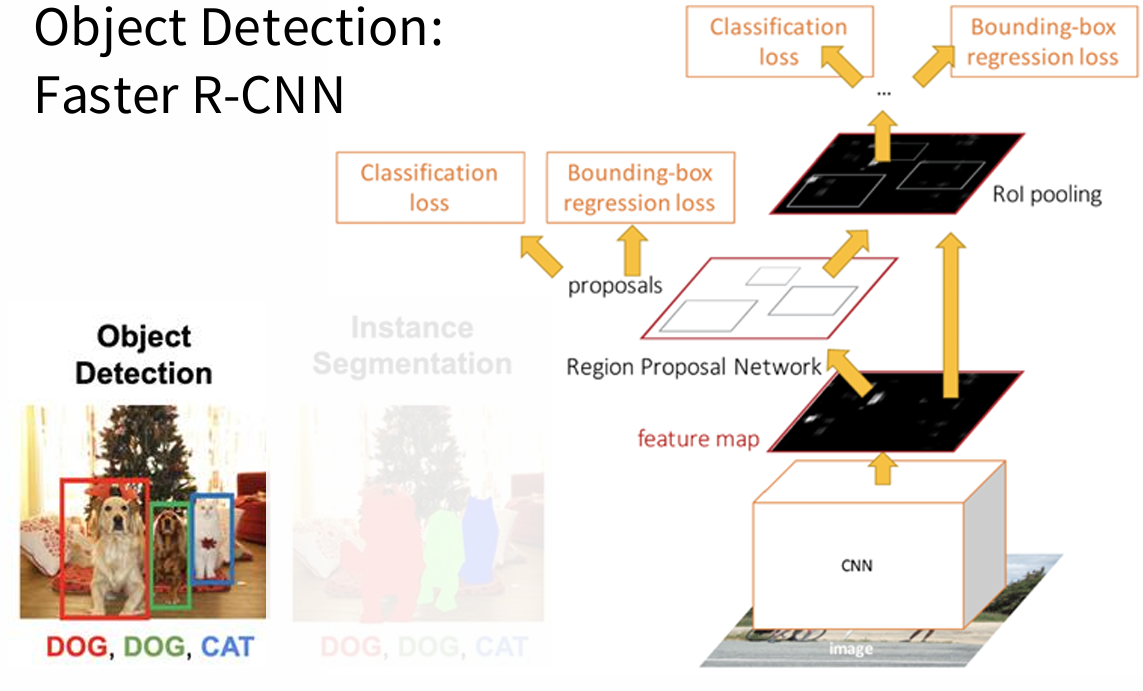
\includegraphics[width=0.9\textwidth]{images/faster_rcnn3.png}
	% Placeholder for: A 3-panel image showing (L) Class, (M) Det, (R) Seg on the same anatomy
\end{frame}

\begin{frame}{Comparison of Object Detection Algorithms}
	\centering
	\scriptsize
	\renewcommand{\arraystretch}{1.5}
	\begin{tabularx}{\textwidth}{|l|X|c|X|}
		\hline
		\textbf{Algorithm}   & \textbf{Features}                                                                                                                                                                                & \textbf{Prediction time / image} & \textbf{Limitations}                                                                                                                                                                 \\ \hline
		CNN                  & Divides the image into multiple regions and then classifies each region into various classes.                                                                                                    & -                                & Needs a lot of regions to predict accurately and hence high computation time.                                                                                                        \\ \hline
		RCNN                 & Uses selective search to generate regions. Extracts around 2000 regions from each image.                                                                                                         & 40-50 seconds                    & High computation time as each region is passed to the CNN separately.                                                     \\ \hline
		Fast RCNN            & Each image is passed only once to the CNN and feature maps are extracted. Selective search is used on these maps to generate predictions. & 2 seconds                        & Selective search is slow and hence computation time is still high.                                                                                                                   \\ \hline
		Faster RCNN          & Replaces the selective search method with the region proposal network.                                                                                      & 0.2 seconds                      & Object proposal takes time.                                                                                                                                                            \\ \hline
	\end{tabularx}
\end{frame}

\begin{frame}{One-Stage Detectors: YOLO}
	\centering

	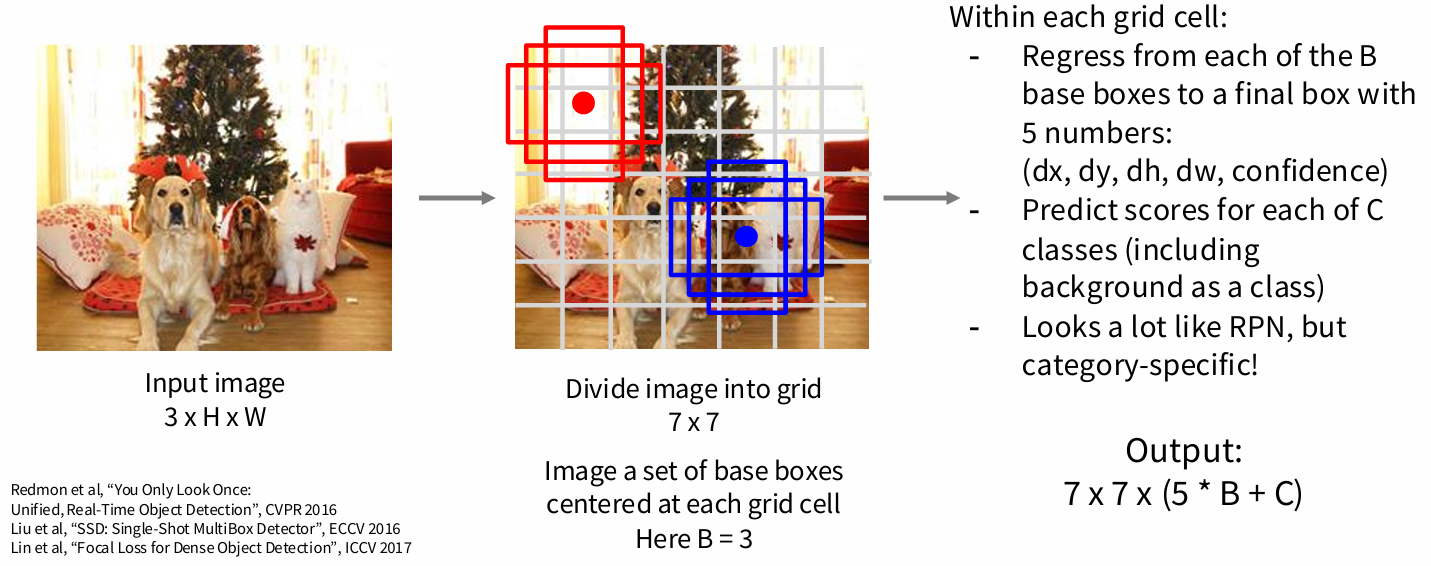
\includegraphics[width=1\textwidth]{images/yolo.png}
	% Placeholder for: A 3-panel image showing (L) Class, (M) Det, (R) Seg on the same anatomy
\end{frame}

\begin{frame}{One-Stage Detectors: YOLO}
	\centering

	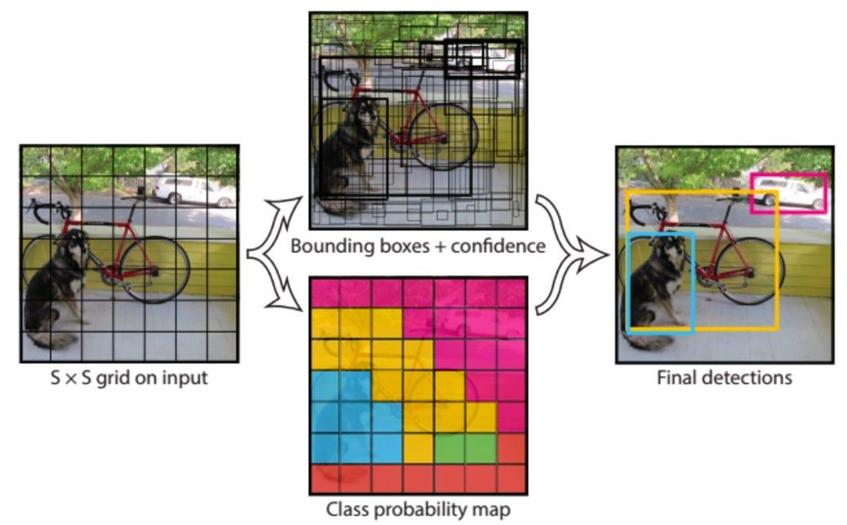
\includegraphics[width=1\textwidth]{images/yolo2.png}
	% Placeholder for: A 3-panel image showing (L) Class, (M) Det, (R) Seg on the same anatomy
\end{frame}

\begin{frame}{One-Stage Detectors: YOLO}
	\centering

	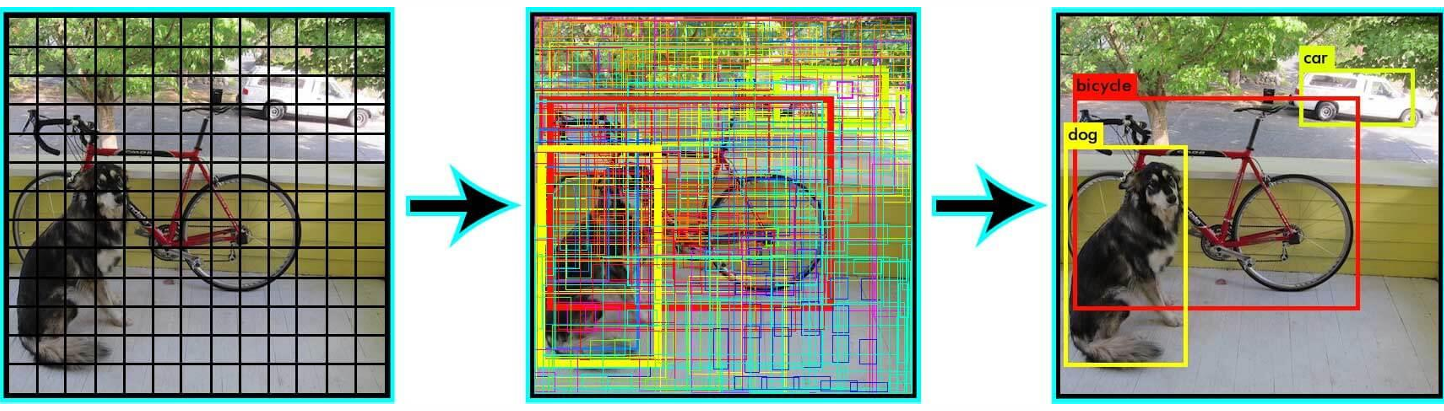
\includegraphics[width=1\textwidth]{images/yolo3.png}
	% Placeholder for: A 3-panel image showing (L) Class, (M) Det, (R) Seg on the same anatomy
\end{frame}

\begin{frame}{One-Stage Detectors: DETR}
	\centering

	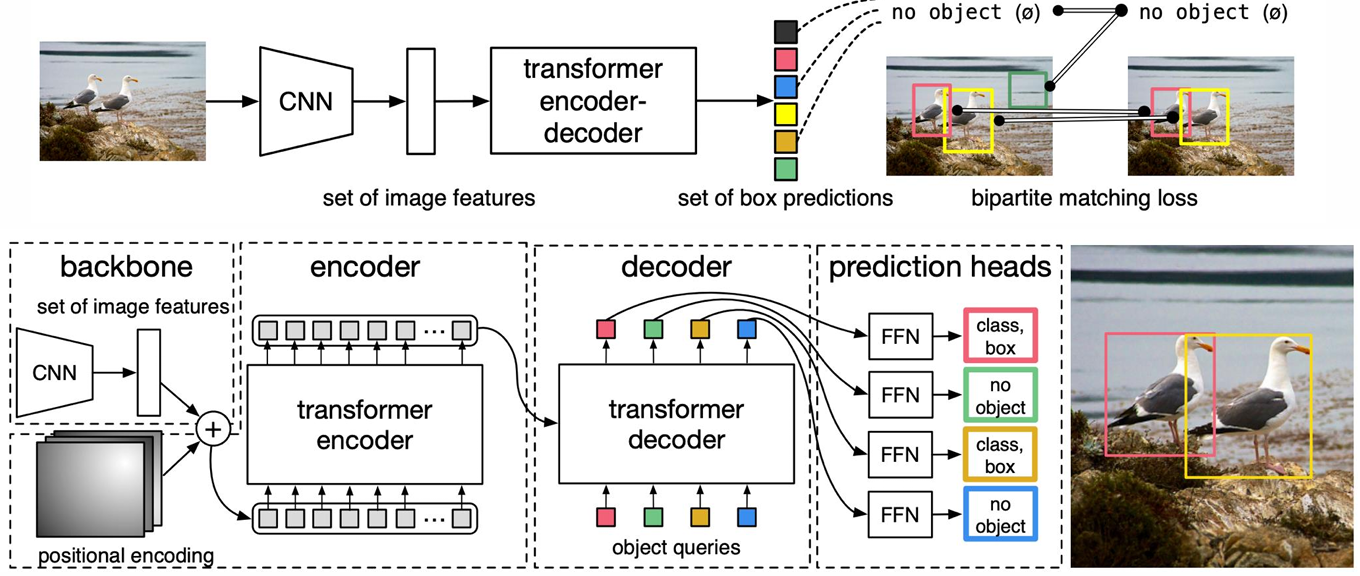
\includegraphics[width=1\textwidth]{images/detr.png}
	% Placeholder for: A 3-panel image showing (L) Class, (M) Det, (R) Seg on the same anatomy
\end{frame}


% ============================================================
\section{Instance Segmentation}
% ============================================================

\begin{frame}{Instance Segmentation}

	\centering

	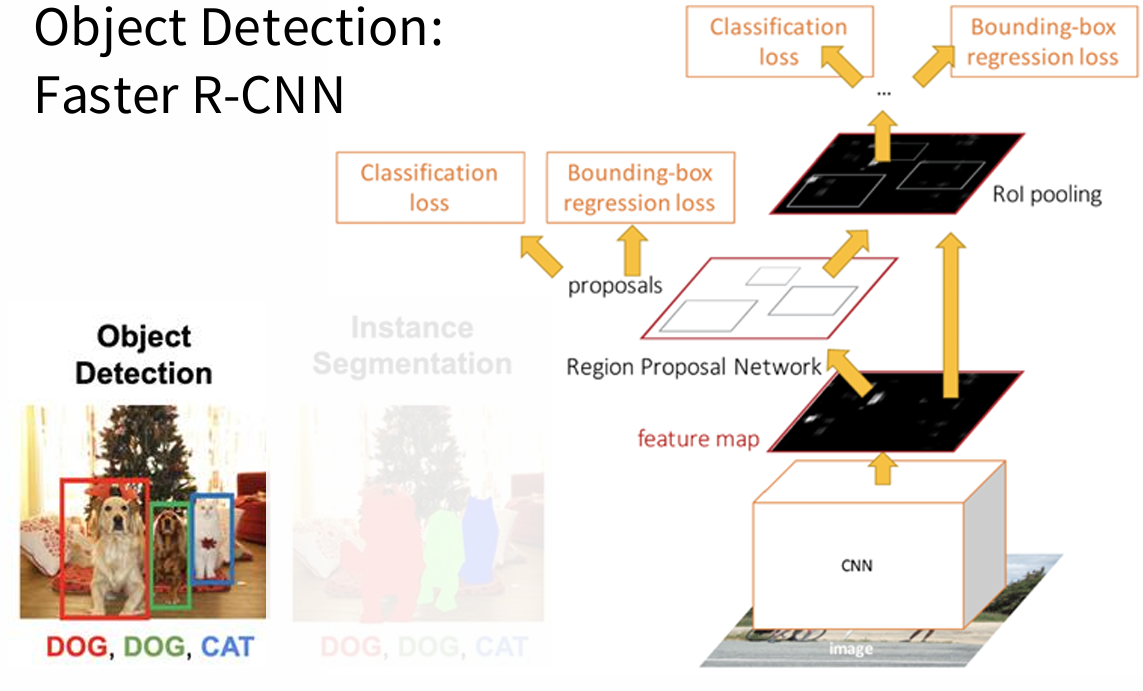
\includegraphics[width=0.9\textwidth]{images/faster_rcnn3.png}
	% Placeholder for: A 3-panel image showing (L) Class, (M) Det, (R) Seg on the same anatomy
\end{frame}

\begin{frame}{Instance Segmentation}

	\centering

	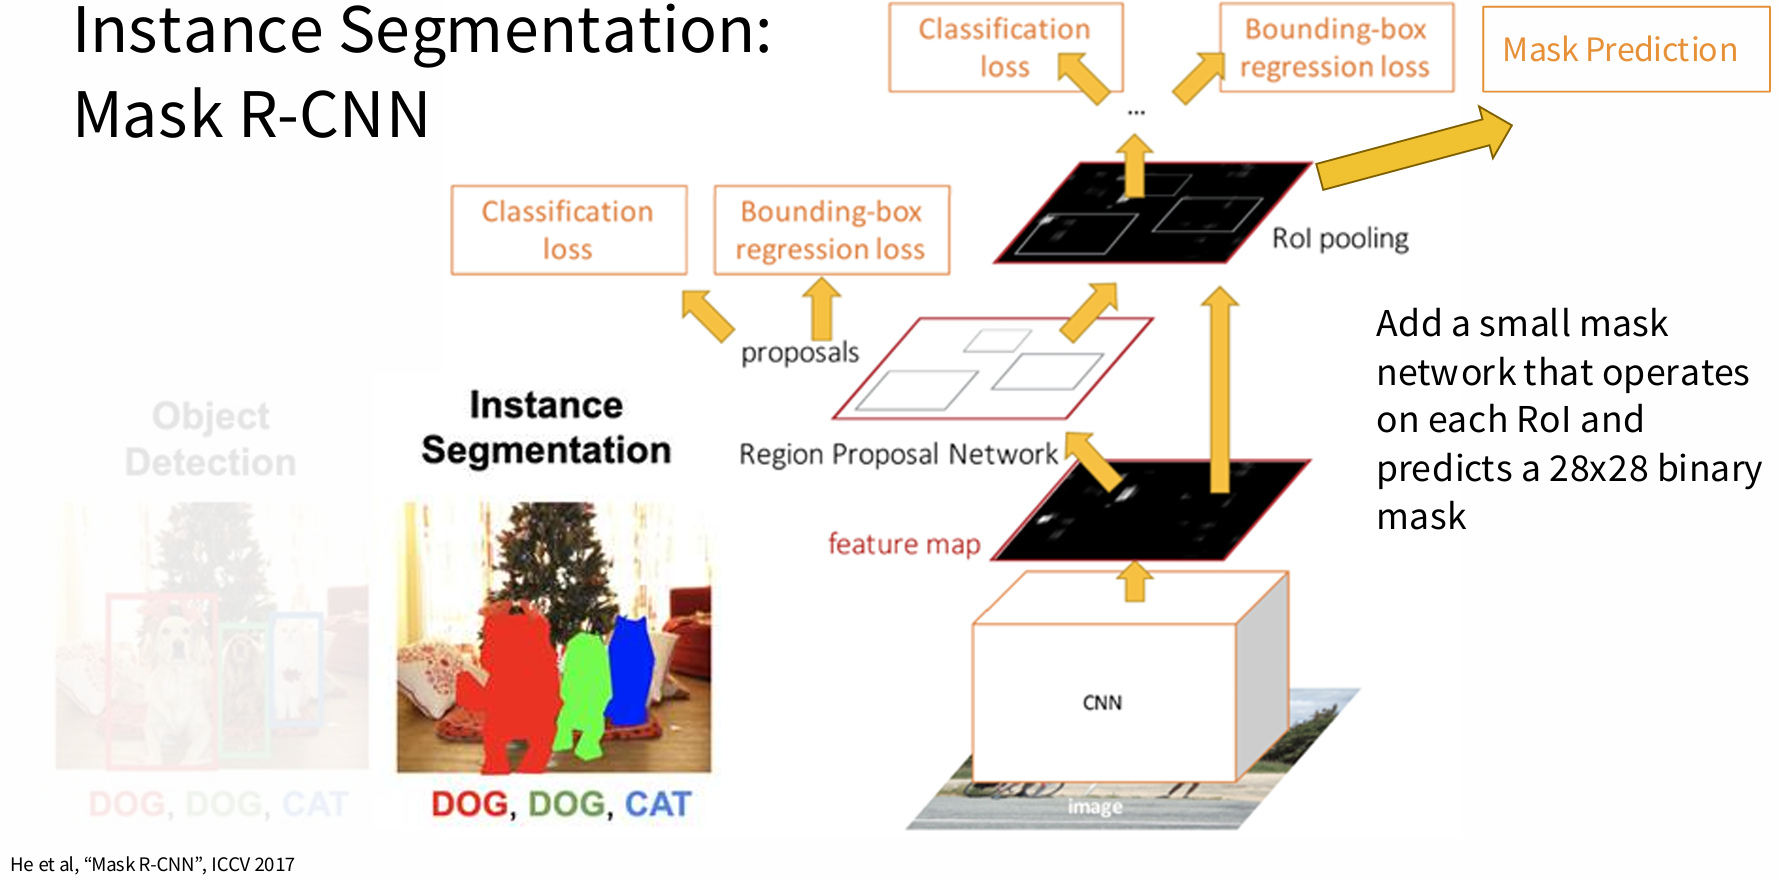
\includegraphics[width=1\textwidth]{images/int_segment.png}
	% Placeholder for: A 3-panel image showing (L) Class, (M) Det, (R) Seg on the same anatomy
\end{frame}

\begin{frame}{Instance Segmentation}

	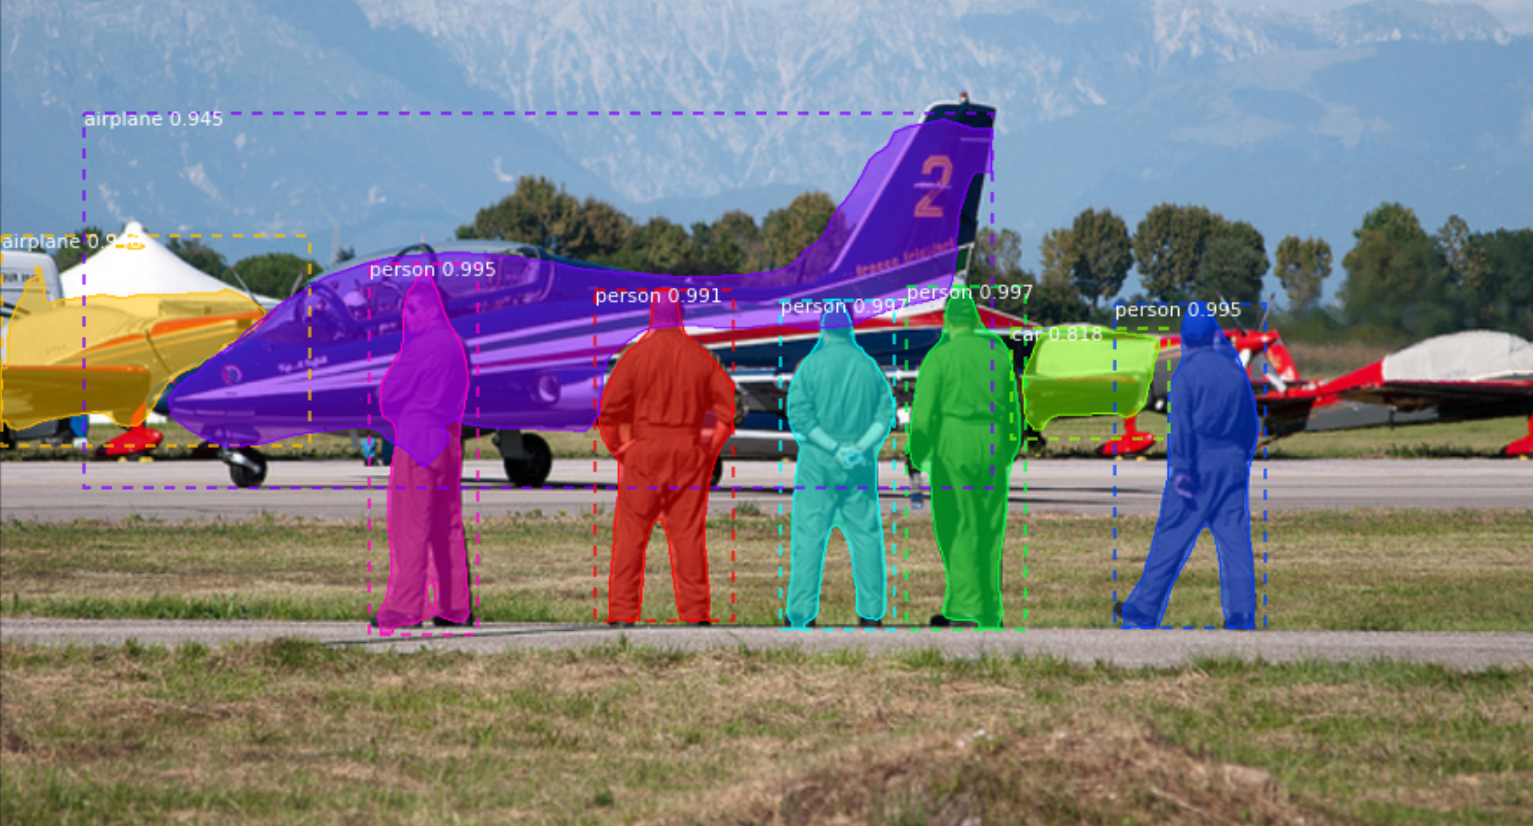
\includegraphics[width=0.9\textwidth]{images/int_segment2.png}
	% Placeholder for: A 3-panel image showing (L) Class, (M) Det, (R) Seg on the same anatomy
\end{frame}

\begin{frame}
	\centering
	\Huge{Thank You!}\\
	\vspace{0.5cm}
	\large{Questions?}
\end{frame}

\end{document}